%-----------------------------------------------------------------------
%
% File Name: thesis.tex
%
% Author: Lough, J. D.
%
%
%-----------------------------------------------------------------------

% document class and packages
\documentclass[12pt,notitlepage]{report}
\usepackage{bibunits}
\usepackage{syrthesis}
\usepackage{graphicx}
%\usepackage{subfigure}
\usepackage{subfig}
\usepackage{array}
\usepackage{multirow}
\usepackage{color}
\usepackage[table]{xcolor}
\usepackage{amsmath}
\usepackage{amssymb}
\usepackage{amsfonts}
\usepackage{tensor}
\usepackage{acronym}
\usepackage{listings}
\lstset{breaklines=true,
  basicstyle=\ttfamily\footnotesize}
\usepackage{lscape}
\usepackage{hyperref}
\usepackage{caption}
%\usepackage{subcaption}
%\usepackage[all]{hypcap}
\usepackage{dsfont}
\usepackage[disable,colorinlistoftodos]{todonotes}
\usepackage{tikz}
\usepackage{pgfplots}
\pgfplotsset{width=14cm,compat=1.6}
\usetikzlibrary{external,shapes,arrows,calc,positioning}
%\tikzexternalize[prefix=tikz/,mode=list and make]
\tikzexternalize[prefix=tikz/]


% journal definitions
\newcommand{\apj}{{\it Astrophysical J.}}
\newcommand{\apjl}{{\it Astrophysical J.}}
\newcommand{\aap}{{\it Astron. and Astrophys.}}
\newcommand{\cmp}{{\it Commun. Math. Phys.}}
\newcommand{\grg}{{\it Gen. Rel. Grav.}}
\newcommand{\cqg}{{\it Class. Quant. Grav.}}
\newcommand{\lr}{{\it Living Reviews in Relativity}}
\newcommand{\mnras}{{\it Mon. Not. Roy. Astr. Soc.}}
\newcommand{\pr}{{\it Phys. Rev.}}
\newcommand{\prl}{{\it Phys. Rev. Lett.}}
\newcommand{\pra}{{\it Phys. Rev. A}}
\newcommand{\prd}{{\it Phys. Rev. D}}
\newcommand{\nat}{{\it Nature}}
\newcommand{\prsl}{{\it Proc. R. Soc. Lond. A}}
\newcommand{\ptrsl}{{\it Phil. Trans. Roy. Soc. London}}
\newcommand{\rmp}{{\it Rev. Mod. Phys.}}
\newcommand{\jcap}{{\it J. Cosmol. Astropart. Phys.}}

% acronymn definitions
\acrodef{LIGO}{Laser Interferometer Gravitational-wave Observatory}
\acrodef{BNS}{binary neutron star}
\acrodef{BBH}{binary black hole}
\acrodef{NSBH}{neutron-star black-hole binary}
\acrodef{FAR}{\emph{false alarm rate}}
\acrodef{IFAR}{inverse false alarm rate}
\acrodef{SNR}{signal-to-noise ratio}
\acrodef{MM}{minimal match}
\acrodef{IFO}{interferometer}
\acrodef{CBC}{compact binary coalesence}
\acrodef{GW}{gravitational wave}
\acrodef{PDF}{probability distribution function}
\acrodef{S5}{LIGO's fifth science run}
\acrodef{S6}{LIGO's sixth science run}
\acrodef{VSR1}{Virgo's first science run}
\acrodef{VSR2}{Virgo's second science run}
\acrodef{VSR3}{Virgo's third science run}
\acrodef{pN}{post-Newtonian}
\acrodef{LVC}{LIGO Scienctific Collaboration and the Virgo Collaboration}
\acrodef{DAG}{directed acyclic graph}
\acrodef{HIPE}{Hierarchical Inspiral Pipeline Executable}
\acrodef{HIPE}{Hierarchical Inspiral Pipeline Executable}
\acrodef{SPA}{stationary-phase approximation}
\acrodef{ISCO}{the inner-most stable circular orbit}
\acrodef{FFT}{Fast-Fourier Transform}
\acrodef{LLO}{LIGO Livingston Observatory}
\acrodef{LHO}{LIGO Hanford Observatory}
\acrodef{LSC}{LIGO Scientific Collaboration}
\acrodef{DQ}{data quality}
\acrodef{LLF}{local Lorentz frame}
\acrodef{GR}{General Relativity}
\acrodef{EM}{electromagnetic}
\acrodef{pdh}[PDH]{Pound Drever Hall}
\acrodef{psl}[PSL]{pre-stabilized laser}
\acrodef{iss}[ISS]{intensity stabilization servo}
\acrodef{fss}[FSS]{frequency stabilization servo}
\acrodef{pmc}[PMC]{pre-mode cleaner}
\acrodef{scs}[SCS]{Sub-Carrier Servo}
\acrodef{ndyag}[Nd:YAG]{neodymium-doped yttrium aluminum garnet}
\acrodef{npro}[NPRO]{non-planar ring oscillator}
\acrodef{aom}[AOM]{accousto-optic modulator}
\acrodef{eom}[EOM]{electro-optic modulator}
\acrodef{pd}[PD]{photo-diode}
\acrodef{daq}[DAQ]{data acquisitions}
\acrodef{daqd}[daqd]{\ac{daq} daemon}
\acrodef{dtt}[DTT]{Diagnostic Test Tools}
\acrodef{asd}[ASD]{amplitude spectral density}
\acrodef{fsr}[FSR]{free spectral range}
\acrodef{fwhm}[FWHM]{full width at half max}
\acrodef{pzt}[PZT]{piezo electric transducer}
\acrodef{psd}[PSD]{power spectral density}
\acrodef{pbs}[PBS]{polarizing beam splitter}
\acrodef{vco}[VCO]{voltage controlled oscillator}
\acrodef{rin}[RIN]{relative intensity noise}
\acrodef{sos}[SOS]{small optic suspension}
\acrodef{rfpd}[RFPD]{radio frequency photodiode}
\acrodef{fi}[FI]{faraday isolator}
\acrodef{qpd}[QPD]{quadrant photodiode}
\acrodef{rms}[rms]{root mean squared}
\acrodef{osem}[OSEM]{optical sensing electro-magnet}
\acrodef{ligo}[LIGO]{Laser Interferometer Gravitational-wave Observatory}
\acrodef{aligo}[aLIGO]{Advanced \ac{ligo}}
\acrodef{wfs}[WFS]{wavefront sensing}

% common macros
\def\Msun{\ensuremath{\mathrm{M_\odot}}}
\def\Mpc{\ensuremath{\,\mathrm{Mpc}}}
\def\yr{\ensuremath{\,\mathrm{yr}}}
\def\mchirp{\ensuremath{\mathcal{M}}}
\def\mtotal{\ensuremath{\mathrm{M_{total}}}}
\def\d{\ensuremath{\,\mathrm{d}}}
\def\pls{\ensuremath{+}}
\def\crs{\ensuremath{\times}}
\def\effD{\ensuremath{\mathcal{D}}}
\def\th{\ensuremath{^{\mathrm{th}}}}
\def\rhonew{\ensuremath{\rho_{\mathrm{n}}}}
\def\rhonewc{\ensuremath{\rho_{\mathrm{nc}}}}
\def\ihope{\texttt{ihope}}
\def\hipe{\texttt{HIPE}}
\newcommand{\lstin}{\lstinline[basicstyle=\ttfamily]}
\newcommand{\todopar}{\todo[inline,color=blue]}
\newcommand{\todoa}{\todo[color=red]}
\newcommand{\todob}{\todo[color=yellow]}
\newcommand{\todoc}{\todo[color=green]}
\newcommand\KB{1.381e-23}
\newcommand\TROOM{295}
\newcommand\PI{3.1415927}
\newcommand\RHOFS{2.2e3}
\newcommand\EEPOXY{3.378e9}
\newcommand{\tcr}{\textcolor{red}}
\newcommand{\tcb}{\textcolor{blue}}
\newcommand{\tcm}{\textcolor{magenta}}
\newcommand{\tcg}{\textcolor{green}}
\newcommand{\tcp}{\textcolor{purple}}
\newcommand{\irm}{\mathrm{i}}


\begin{document}

\Abstract{

The Advanced LIGO detectors will soon be online with enough sensitivity to
begin detecting gravitational waves,
based on conservative estimates of the rate of
neutron star inspirals.
These first detections are sure to be significant, however, we will always
strive to do better. More questions will be asked about the nature of
neutron star material, rates of black hole inspirals, electromagnetic
counterparts, etc.
To begin to answer all of the questions aLIGO will bring
us we will need even better sensitivity in future gravitational wave
detectors.

This thesis addresses one aspect that will limit us in the future:
angular stability of the test masses.
Angular stability in advanced LIGO uses an active feedback system.
We are proposing to replace the active feedback system with a passive
one, eliminating sensing noise contributions.
This technique uses the radiation pressure of light inside a cavity as a
stable optical spring, fundamentaly the same as technique developed by
Corbitt, et al. \cite{Corbitt07} with an additional degree of freedom.

I will review the theory of the one dimensional technique and discuss the
the multidimensional control theory and angular trap setup.
I will then present results from the one-dimensional trap which we have
built and tested. And propose improvements for the angular trap experiment.

Along the way we have discovered an interesting coupling with thermal
expansion due to round trip absorption in the high reflective coatings.
The front surface HR coating limits our spring stability in this experiment
due to the high circulating power and small beam spot size.


}

\title{
Optical Spring Stabilization
}
\author{James D. Lough}
\pastdegrees{B.S. Virginia Tech, 2001}
\majorprof{Advisor}
\submitdate{December 2014}
\degree{Doctor of Philosophy}
\program{Physics}
\copyrightyear{2014}

\majordept{Physics}
\havededicationtrue
\dedication{to\\my little scientists,\\Elizabeth and Henry}
\haveminorfalse
\copyrighttrue
\doctoratetrue
\figurespagetrue
\tablespagetrue
\signedtitlepfalse

\beforepreface \prefacesection{Preface}

The thesis presented here would not have been possible without collaboration
with my colleagues.
First, and foremost, the main subject of this thesis is the optical trap
experiment taking place at Syracuse University.
Much of the work in setting up the experiment was done together and will
be difficult to differential exact contributions from members.

This experiment was very much a combined effort of primarily four people:
our PI Stefan Ballmer, David Kelley, Antonio Perreca, and myself.
We were fortunate to have some major infrastructure in place when we started:
two large vacuum bell jars, two optics benches with floating legs.
The rest of the experiment was pretty much built from the ground up.

Another graduate student, Fabian Magana-Sandoval recently joined our team
and has contributed to the building of \ac{qpd}s and the commissioning of the
optical lever.

There has also been contributions from other graduate students as part of
requirements for the course Graduate Laboratory:
\begin{itemize}
\item Prayush Kumar designed the \ac{iss}.
\item Alex Nitz worked on the \ac{pmc}.
\item Chris Biwer is adding a feedforward modification to the \ac{pmc}.
\end{itemize}
Also, my work on building and commissioning the \ac{iss} was for fulfillment of the
grad lab course.

My major contributions to the experiment have been:
\begin{itemize}
\item setting up the vacuum system infrastructure and electrical feedthroughs,
\item designing and building the reference cavity and suspension for the
  \ac{fss},
\item designing the trap output mirror "payload" suspension,
\item assembling the digital control system,
\item and assembling and commissioning the suspension control loops.
\end{itemize}

The theory presented in chapter \ref{ch:theory} is primarily copied from our
group's recent paper, Multidimensional optical trapping of a mirror,
Perreca et al. \cite{Perreca:2014}

%The work presented in this thesis stems from my participation in the LIGO
%Scientific Collaboration and the Virgo Collaboration.
%
%A bit of LIGO history and motivation for LIGO itself.
%
%What lies ahead?
%
%Future of radiation pressure applications.

%\prefacesection{Conventions}
%
%Mirror reflectivities are designated by $r$ for the amplitude reflectivity
%and $R$ for the power reflectivity.
%I will use $\mathcal{R}$ for radius of curvature,
%but the distinction should be apparent in the context.



%We use the Einstein summation convention in which repeated upper and lower
%indices are summed over. Greek indices indicate all four spacetime dimensions,
%Latin indicate spatial dimensions only. An over-arrow indicates a vector with
%spatial components only, e.g., $\vec{x} = (x^1,x^2,x^3)$.
%
%\vspace{0.5cm}
%
%\noindent Expectation values of a variable are indicated by $\mathbb{E}()$.
%Averages, unless otherwise noted, are indicated by an overbar.
%
%\vspace{0.5cm}
%
%\noindent The time-stamps of interferometer data are measured in
%Global Positioning System (GPS) seconds: seconds since 00:00.00 UTC
%January 6, 1980 as measured by an atomic clock.

\prefacesection{Acknowledgments}
% $Id$

As a member of the LIGO Scientific Collaboration, I have been fortunate to
have benefited through advice from and discussions with many people. It would
not be possible to thank everyone who I have worked with over the past five
years without making the acknowlegements longest chapter in this dissertation,
so I shall only attempt to thank those who I have interacted with the most and
hope that the others forgive me.

First and foremost, I would like to thank Patrick Brady. I am fortunate to
have an advsior whose as big a drunk as I am.

I would also like to thank Jolien Creighton for his help and enthusiasm over
the past five years. It has been fun working with Jolien and I have learnt a
great deal from him through his patient explanations.

I am greatful to Bruce Allen for suggesting the search for binary inspiral as
a research topic and his assitance with the scientific and computational
obstacles along the way. Thanks also to Gabriela Gonz\'{a}lez for patiently
anserwing my many stupid questions about the LIGO interferometers helping me
understand the data that I have been analyzing.

I would like to thank the members of my committee: Daniel Agterberg, John
Friedman and Leonard Parker for their careful reading of this dissertation and
helpful suggestions for its improvement.

I also would like to thank Warren Anderson, Teviet Creighton, Stephen
Fairhurst, Scott Koranda, Eirini Messaritaki, Ben Owen, Xavier Siemens and
Alan Wiseman for help, advice and pints of beer. I am also indebted to Axel's
for many useful discussions.

Thanks to Steve Nelson, Wyatt Osato and Quiana Robinson for their help in the
preparation of this this and, of course, to Sue Arthur for making everything
run smoothly.

I could not have come this far without the constant love and support of my
parents, to whom this thesis is dedicated. Finally, I would like to thank
Emily Dobbins for all the love and understanding over the past two years.


\afterpreface

\listoftodos

%\Chapter{Document Planning}
%\label{ch:planning}
%\input{todos.tex}

\Chapter{Introduction}
\label{ch:introduction}
In 1915, Albert Einstein published his theory of general relativity, a 
geometric theory of gravitation that sought to expand upon Newtonian 
mechanics and provide a complete description of gravity and its 
relationship with space and time. Einstein theorized that space 
and time were deeply related and existed together as a manifold 
called spacetime. Matter with energy and momentum 
existing in this manifold would create 
curvature in spacetime. Gravitational forces were the result of 
matter following geodesic curves in spacetime. This concept can 
be summarized in the Einstein field equation, which is presented 
as,
\begin{equation}
G_{\mu\nu} = 8\pi T_{\mu\nu}
\label{eq:EFE}
\end{equation}
where $G_{\mu\nu}$ is the Einstein tensor, which describes the 
curvature of spacetime, $T_{\mu\nu}$ is the 
stres-energy tensor, which describes the energy and momentum in 
spacetime, and  $G=c=1$. The Einstein tensor is defined as,
\begin{equation}
G_{\mu\nu} = R_{\mu\nu} - \frac{1}{2}Rg_{\mu\nu}
\end{equation}
where $R_{\mu\nu}$ is the Ricci curvature tensor and $g_{\mu\nu}$ is 
the metric tensor for the manifold.

An interesting result that arises from this formalism is the 
existence of gravitational waves, which are perturbations in 
spacetime caused by certain types of time-varying mass distributions. 
To describe gravitational waves, we consider 
a Minkowski metric with a small perturbation. The Minkowski metric 
is a flat spacetime metric defined as
\begin{equation}
\eta_{\mu\nu} = 
  \begin{pmatrix}
   -1 & 0 & 0 & 0 \\
    0 & 1 & 0 & 0 \\
    0 & 0 & 1 & 0 \\
    0 & 0 & 0 & 1
  \end{pmatrix}
\end{equation}
where $\mu = 0$ corresponds to the time coordinate and $\mu = {1,2,3}$ 
correspond to the spatial coordinates. In examples, we will use the coordinate 
convention $(x^0,x^1,x^2,x^3) = (ct,x,y,z)$. 
The full spacetime metric, $g_{\mu\nu}$, is then constructed as a 
linear perturbation on the Minkowski metric,
\begin{equation}
g_{\mu\nu} = \eta_{\mu\nu} + h_{\mu\nu}
\end{equation}
where $h_{\mu\nu}$ is the metric perturbation and $|h_{\mu\nu}| \ll 1$.
From here, we follow the convention of Saulson \cite{Saulson:1994} to arrive at the general 
form of a gravitational wave.
At this point it is very useful to move into the transverse traceless 
gauge where coordinates on the manifold are defined by the geodesic 
motion of freely-falling test masses. In this gauge, the weak field 
vacuum solution of the Einstein field equation becomes a wave equation: 
\begin{equation}
\square h_{\mu\nu} = 0.
\end{equation}
The solutions to this differential equation will be plane waves of 
the form
\begin{equation}
h_{\mu\nu} = C_{\mu\nu}e^{i(2\pi ft - \vec{k}\cdot\vec{x})}
\end{equation}
where $C_{\mu\nu}$ is the wave amplitude, $f$ is the frequency, 
and $\vec{k}$ is the wave vector which indicates the direction of 
propagation \cite{Carroll}.

For example, consider the case of a gravitational 
wave propogating along the $\hat{z}$-axis.
When the conditions of the transverse traceless gauge are applied, 
the resulting form of $h_{\mu\nu}$ is 
\begin{equation}
h_{\mu\nu} = 
  \begin{pmatrix}
    0 & 0 & 0 & 0 \\
    0 & h_+ & h_x & 0 \\
    0 & h_x & -h_+ & 0 \\
    0 & 0 & 0 & 0
  \end{pmatrix}
\end{equation}
where the diagonal and off-diagonal terms represent two polarizations 
of the resulting gravitational wave, called "h-plus" and "h-cross" 
respectively.
We can see the effects of this perturbation by observing the  
spacetime interval on the manifold. The spacetime interval is defined as 
\begin{equation}
ds^2 = dx^\mu g_{\mu\nu}dx^\nu.
\end{equation}
Substituting in our perturbed metric for $g_{\mu\nu}$, we find that 
the spacetime interval can be broken up into a standard Minkowski line 
element and a perturbation due to $h_{\mu\nu}$.
\begin{equation}
ds^2 = dx^\mu (\eta_{\mu\nu} + h_{\mu\nu})dx^\nu \\
\end{equation}
\begin{equation}
ds^2 = dx^\mu \eta_{\mu\nu} dx^\nu + dx^\mu h_{\mu\nu}dx^\nu
\label{eq:spacetime}
\end{equation}

As an example, we present the case of a plus-polarized gravitational wave 
propagating in the $\hat{z}$ direction and observe the effect of the perturbation 
on the spacetime interval. The perturbation will have the form 
\begin{equation}
h_{\mu\nu} = 
  \begin{pmatrix}
    0 & 0 & 0 & 0 \\
    0 & h_+ & 0 & 0 \\
    0 & 0 & -h_+ & 0 \\
    0 & 0 & 0 & 0
  \end{pmatrix}
\end{equation}
Using the coordinate convention of $(ct,x,y,z)$, the unperturbed
spacetime interval is given as: 
\begin{equation}
ds^2 = -c^2 dt^2 + dx^2 + dy^2 + dz^2.
\end{equation}
Since the perturbation is spatially transverse to the direction of 
propagation, the ct- and z-coordinates will not be modulated by the 
gravitational wave. The x- and y-coordinates will be modulated  
according to equation \ref{eq:spacetime}. The resulting spacetime 
interval is
\begin{equation}
ds^2 = -c^2 dt^2 + (1 + h_+)dx^2 + (1 - h_+)dy^2 + dz^2.
\end{equation}
This shows that a gravitational wave propogating along the $\hat{z}$-axis 
will differentially stretch and squeeze spacetime in the transverse 
axes. The exact form of $h_+$ will depend on the source of the 
gravitational waves. A visualization of this stretching and squeezing 
is shown in Figure \ref{fig:polarizations}\cite{Polarization}. The cross polarization  
stretches and squeezes at a 45 degree angle relative to the plus 
polarization.

\begin{figure}[ht!]
\includegraphics[width=\textwidth]{figures/introduction/polarisations2}
\caption[Plus and cross polarizations]{Plus and cross polarizations %
         of a gravitational wave.}
\label{fig:polarizations}
\end{figure}

The Advanced LIGO interferometers are designed to be sensitive 
to this differential stretching and squeezing by constructing orthogonal 
optical cavities. A gravitational wave passing through an aLIGO interferometer 
will differentially 
modulate the lengths of the optical cavities, creating an interference 
pattern at the output of the instrument that can be searched for 
gravitational wave signals. The layout and gravitational wave readout scheme 
of the interferometers is discussed below.

\section{The Advanced LIGO Interferometers}\label{sec:aligo}

The Advanced LIGO (aLIGO) interferometers are a pair of dual-recycled Michelson interferometers 
that employ 4km long Fabry-Perot cavities in their arms to increase the interaction time with a 
gravitational wave signal. 
Figure \ref{fig:aligo} shows a simplified layout of an aLIGO interferometer. 

\begin{figure}[ht!]
\includegraphics[width=\textwidth]{figures/introduction/ALIGO_layout}
\caption[Layout of Advanced LIGO]{Layout of Advanced LIGO}
\label{fig:aligo}
\end{figure}

At the input to an aLIGO interferometer is a solid-state Nd:YAG laser that provides laser light 
at a wavelength of 1064 nm. Not included in Figure \ref{fig:aligo} are frequency and 
intensity stabilization control loops designed to provide as stable a laser source as 
possible for the experiment. This stabilized laser is called the pre-stabilized laser 
(PSL). The laser light is passed through a series of 
electro-optic modulators (EOM) where radio-frequency (RF) sidebands are generated 
and imparted onto the light. These RF sidebands are used to control auxiliary optical 
degrees of freedom in the interferometer. The beam is then passed through the 
input mode cleaner (IMC), which rejects higher order spatial modes of the beam 
and transmits a circular TEM00 mode to be used in the instrument.

Once the beam has been stabilized in frequency and intensity and the higher order 
optical modes have been stripped away, it is transmitted through the power 
recycling mirror and enters the vertex of the interferometer. In the vertex, 
the beam is split 50/50 by the beamsplitter. Half of the light is directed toward  
the input test mass (ITM) of the X-arm and half of the light is directed  
toward the ITM of the Y-arm. As mentioned previously, the aLIGO arms are not 
single bounce cavities; they are comprised of Fabry-Perot cavities that allow the 
light to circulate in the arm cavities multiple times. The light is stored in 
the arm cavities for $\sim$1ms, trapped between the highly reflective surfaces 
of the ITM and the end test mass (ETM), before it is transmitted back through 
the ITM and into the vertex.

When a gravitational wave passes through an aLIGO inteferometer, the distance
between the ITM and ETM of each arm is modulated, causing the light to have a
longer or shorter travel time as it traverses the arm. Since gravitational
waves expand space in one direction while the orthogonal direction contracts,     
the X- and Y-arms will experience differential changes in length. When light
from the arms is recombined at the beamsplitter, there will be a difference
in phase between the two beams as they have traveled different paths. The 
resulting light from this recombination of phase shifted beams is called the 
antisymmetric part of the output. The part of the beam that is recombined 
in phase is called the symmetric part of the output.

The beams returning from each arm are recombined at the beamsplitter. The 
symmetric part of the beam 
will be sent back toward the power recycling mirror. The power recycling mirror 
forms a resonant cavity with the ITMs, allowing for light at the symmetric 
port of the beamsplitter to be added coherently to incoming light from the PSL and 
increasing the effective power in the vertex. This increase in effective power 
is known as the power recycling gain. 

The antisymmetric part of the beam is sent toward the signal recycling mirror. 
The signal recycling cavity is used to tune the frequency response of the 
interferometer by adjusting the effective finesse of the coupled cavity 
formed by the signal recycling cavity and the arm cavities. 
If the light returning from the arms has accumulated some differential amount of 
phase as it traveled 
along the arms, perhaps from a gravitational wave modulating the length of each 
arm differentially, it will be transmitted through the signal recycling cavity 
and into the output mode cleaner (OMC). The OMC behaves similarly to the IMC, 
stripping away higher order optical modes and isolating the TEM00 mode of the 
beam. The transmitted, mode cleaned signal is then read out using a homodyne 
detection scheme on a DC photodiode. 

\subsection{DC Readout}

When a gravitational wave modulates the length of an arm cavity, the light 
traveling in that arm experiences a phase modulation. This phase modulation 
can be visualized by picturing the beam in frequency space. In figure 
\ref{fig:omc-freq}, the carrier beam frequency is designated as $f_0$. 
The phase modulation due to 
a gravitational wave signal introduces a frequency sideband at the 
gravitational wave frequency, which is in the 30-2000 Hz range. 
The 
RF sidebands used for auxiliary optical cavity control are offset from the 
carrier frequency by 9, 24, and 45 MHz. 
The RF sidebands, which in a 
homodyne detection scheme would only contribute shot noise to the output signal, 
are rejected by the OMC. The gravitational wave sidebands, however, are at a 
low enough frequency offset that they are within the cavity pole of the OMC 
and are allowed to transmit through the cavity.

Since the OMC DC photodiode measures power, it measures the square of the 
incident optical field and witnesses beat frequencies between different 
components of the light. If the RF sidebands have been filtered out by 
the OMC, the only remaining beat note will be that of the carrier beam ($f_0$) 
beating against the gravitational wave sideband ($f_0 + f_{GW}$). This beat note will 
appear as the difference in frequency between the two optical fields, 
leaving behind a signal in the 30-2000 Hz range ($f_{GW}$) and providing a 
natural demodulation inherent to the measurement process. 
The process of recovering the gravitational wave sideband using the 
carrier field as a reference is known as homodyne detection. 

\begin{figure}[ht!]
\includegraphics[width=\textwidth]{figures/introduction/omc-freq}
\caption[Sidebands and OMC cavity pole]{Frequency domain visualization of beam %
         at OMC. Grey dotted lines indicate the cavity pole. The gravitational %
         wave sidebands are within the cavity pole and are transmitted through %
         the OMC. The RF sidebands are in the MHz range and are rejected by the %
         OMC.}
\end{figure}\label{fig:omc-freq}

\section{Sources of Gravitational Waves}
Include that box with modeled, unmodeled, transient, and continuous.

CBCs are the bread and butter, expect BNS, NSBH, and BBH sources
Continuous waves from pulsars
Bursts from supernovae
Stochastic background


\section{Searching for Compact Binary Coalescences}

Steal this from O1 CBC DQ paper


\section{The Advanced Detector Network}

The Advanced Laser Interferometer Gravitational-Wave Observatory (aLIGO) is 
part of a worldwide effort to detect gravitational waves from astrophysical 
sources. The two aLIGO interferometers, one in Hanford, WA and one in 
Livingston, LA, are part of a growing network of ground-based interferometric 
gravitational wave detectors. Each aLIGO interferometer has 4km long arms 
arranged in an L-shaped configuration. A gravitational wave passing through 
an aLIGO interferometer will cause the arms to expand and contract, 
creating an interferometric signal at the output of the instrument. 
Section \ref{sec:aligo} contains a more detailed description of the aLIGO 
interferometers. 

There are a number of other interferometric gravitational wave detectors 
being built and commissioned for future use in collaboration with aLIGO.
The Advanced VIRGO detector is being built and commissioned in Cascina, Italy. 
When it is fully commissioned, VIRGO will be joining LIGO in observing runs. 
The VIRGO interferometer has 3km arms, which should provide enough 
sensitivity to allow for triangulation of astrophysical sources.

The GEO600 detector, located in Hanover, Germany is an interferometer built in 
collaboration between Germany and the United Kingdom. 
GEO600 is an extremely valuable test bed for interferometric technologies,
including quantum optics and homodyne detection. However, with 600m arms, GEO600 
is unlikely to be sensitive enough to witness expected astrophysical sources.

The KAGRA detector, located underground in the Kamioka mine in Japan, 
is in its commissioning phase. KAGRA has 3 km long arms and, 
unlike other gravitational wave interferometers, employs cryogenics to 
reduce thermal noise in its optics. When complete, KAGRA should be 
sensitive enough to contribute to the worldwide detector network.

Include that cool picture of the advanced detector network.


%\Chapter{Angular Noise in LIGO Detectors}
%\label{ch:anglenoise}
%\section{Optical Cavities and Radiation Pressure}

\section{Sidles-Sigg Instabilities}

\section{Current Stabilization Methods}



%\Chapter{Optical Spring Stabilization}
%\label{ch:opspringstab}
%As discussed in chapter \ref{ch:introduction}, a Fabry-Perot cavity of just the right
length can support a resonant laser field. If this cavity were to be slightly longer or
shorter, the power buildup inside the cavity will fall. The power buildup in the cavity
produces a force due to radiation pressure which pushes against the end mirrors
of the cavity. This force is length dependent, the first order of which gives a spring
term. Clearly, one can see that if the cavity is detuned slightly from resonance a
spring is created. We call this an optical spring.

\Chapter{Angular Optical Trap}
\label{ch:theory}
In this chapter I will cover the theory necessary for the angular optical trap
which we are striving for and which the Syracuse linear trap is the first major
step on the road.

This chapter is mostly excerpts from the paper which provides the theory and
motivation for the angular optical trap experiment.\cite{PhysRevD.89.122002}
Sections \ref{sec:II},\ref{sec:III},\ref{sec:IV}, and \ref{sec:V} are copied
directly from this paper.


\section{Stability principle}
\label{sec:II}
%Firstly we consider the trap mirror as a suspended mirror located at the end of a Fabry-Perot cavity. 
%Dual carrier approach for mirror position control is based on the use of a strong (carrier) and a weak
%(subcarrier) field created to form two optical springs in such a way to have a stable system when 
%summed to the mechanical spring. %An additionally couple of beams need to be used for the angular control.

An optically detuned Fabry-Perot cavity naturally leads to a linear coupling between intra-cavity power and 
mirror position. Depending on the sign of the detuning, this coupling creates an optical spring which
is either statically stable or unstable. Due to the time delay in the optical field build-up, the optical spring 
restoration force is slightly delayed. This leads to a dynamically unstable spring for the statically stable case
and a dynamically stable spring for the statically unstable case. Corbitt et. al. \cite{Corbitt07} demonstrated that by adding a second, frequency-shifted optical field (sub-carrier) with a different detuning and power, a statically and dynamically stable optical spring can be achieved. The dual-carrier scheme has been used to optically trap a gram-scale mirror, controlling its longitudinal degree of freedom.
%thus creating an optical trap for the length degree of freedom of the mirror. 
Moreover, the damping of the optical spring can be controlled by adjusting the detuning of both carrier and sub-carrier and their relative amplitudes. This naturally allows for efficient cooling of the degree of freedom seen by the optical spring. In contrast to a mechanical spring, this damping does not introduce intrinsic losses, and thus does not contribute to the thermal noise.

This technique can be extended to alignment degrees of freedom. By duplicating the Corbitt et al. approach for trapping 
with a second, different, optical axis and a different beam spot on the controlled mirror, it is possible to control the angular 
degree of freedom with radiation pressure alone.
%, thus by-passing the Sidles-Sigg instability.

To be able to understand the stability of multi-dimensional opto-mechanical systems, we first recall the simple driven damped mechanical oscillator. From there we will stepwise increase the complexity by adding optical springs and additional degrees of freedom. 
%\tcr{Following we recall some of the features of a driven mechanical damped oscillator, we introduce the mathematical form of a optical spring and its relation with a mechanical oscillator in terms of control system model.}

%This lead us to the use of a two carrier scheme for the control of a single degree of
%freedom and to a double two carriers scheme for the control of two degrees of freedom.

%%%%%%%%%%%%%%%%%%%%%%%%%%%%%%%%%%%%%%%%%%%%%%%%%%%%%%%%%%%%%%
\subsection{Damped mechanical oscillator stability}
%%%%%%%%%%%%%%%%%%%%%%%%%%%%%%%%%%%%%%%%%%%%%%%%%%%%%%%%%%%%%%

Although the damped mechanical oscillator is a well known system, we will take it as a starting point to make the reading clearer. Our goal is to describe the mechanical oscillator in the language of control theory, which allows us to understand the stability of the system from a different point of view. This approach can then be naturally extended to include the effect of additional optical springs. 

The motion of a harmonic oscillator of mass $m$, spring constant $k_m$ and velocity damping $b$, driven by the external force $F_{ext}$, can be expressed as \cite{Saulson90}:
\begin{eqnarray}
\label{eqn:motion}
m\ddot{x}=-k_m x-b\dot{x}+F_{ext}
\end{eqnarray}
$b$ is also called the viscosity coefficient. Often the damping rate $\Gamma=b/(2 m)$ is used instead.
Traditionally the equation of motion \ref{eqn:motion} is directly used to get the system's position response $x$ when applying the external force $F_{ext}$. The resulting transfer function is
%For such a purpose and for completeness  we can describe the mechanical oscillator in two different way. 
%Both ways are self-consistent.
%One way is to consider the system as a mass with a mechanical spring that moves of the quantity $x$ when subjected at
%the force $F_{ext}$. The law that link the output $x$ and the input $F_{ext}$ of the system is
%given by the transfer function which can be directly obtained by the equation of motion (\ref{eqn:motion}):
%We consider such a system as free-test mass 
%\begin{figure}[htbp]
%	\centering
		%\includegraphics[width=6cm]{./images/Spring_add.eps}
%		\includegraphics[width=5cm]{./images/block_1.eps}
%	\caption{bla bla bla}
%	\label{cavity_k}
%\end{figure}

%That leads to the following transfer function:
\begin{eqnarray}
\label{eqn:TF}
G=\frac{x}{F_{ext}}=\frac{1}{-m\Omega^2+k_m+ib\Omega}                                                 %=\frac{1}{ms^2+b s+k_m}
\end{eqnarray}
with $\Omega$ being the angular frequency of the motion.
% and $s=i\Omega$ being a complex variable. % and $\Gamma=b/m$ is the damping rate. 

Alternatively we can describe a damped mechanical oscillator as a feedback system,  with the plant being just a free-test mass described by the transfer function 
$M=x/F_{ext}=-1/m\Omega^2$,
%Another way that can be used to describe a damped mechanical oscillator is to consider it as
%a feedback system where its plant is just a free-test mass described by the transfer function 
%$M=x/F_{ext}=-1/m\Omega^2$, 
obtained directly from the equation of motion of a free test-mass. 
The control filter of the feedback loop is the mechanical spring, which takes the mass displacement $x$ as input and acts on the plant with the control signal, or force, $F_K$, which is subtracted from the external force $F_{ext}$.
The transfer function of the control filter is $K_M=F_{K}/x=k_m+ib\Omega$. In this picture we can now calculate the closed loop transfer function and obtain the same expression as in equation \ref{eqn:TF}:
\begin{eqnarray}
\label{eqn:TF_fm}
G=\frac{M}{1+K_M M}=
%\frac{\frac{-1}{m\Omega^2}}{1-\frac{K_M}{m\Omega^2}}=
\frac{1}{-m\Omega^2+k_m+ib\Omega}
\end{eqnarray}
where $OL_M=-K_M  M = (k_m+ib\Omega)/m\Omega^2$ describes the open loop transfer function of the system.

%\begin{figure}[htbp]
%	\centering
%		%\includegraphics[width=6cm]{./images/Spring_add.eps}
%		\includegraphics[width=8cm]{./images/blocks}
%	\caption{{(Left)} A damped mechanical oscillator seen as system subjected to the external 
%	force $F_{ext}$ and corresponding displacement $x$ as output.
%	{(Right)} A damped mechanical oscillator seen as a closed-loop system, where the plant $M$
%	is a free-mass, the output is the displacement $x$ which is fed-back to the system through the elastic force $F_k= -K_M \cdot x$ and the input is $F_{ext}-F_{k}$.}
%	\label{fig:blocks}
%\end{figure}

\subsubsection*{Stability}
We can now check for the stability of the system in both pictures.
%The stability of the system related to the two different descriptions can be evaluated in a different manner.
%While the stability in the first description can be evaluated by looking at the poles of its transfer function, the latter
%offers the additional chance to look at its open loop transfer function $M\cdot K_M$ to evaluate its stability.
We recall from literature that the stability of a system described by its transfer function $G$ can be evaluated looking at the poles 
of its transfer function in the s-plane ($s=i\Omega$) \cite{Greensite70}. In particular a system is stable only if its transfer function's poles have
a negative real part,  and the multiplicity of poles on imaginary axis is at most 1.
The transfer function in equation \ref{eqn:TF} has the following poles:
\begin{eqnarray}
\label{eqn:poles}
i\Omega=-\frac{b}{2m}\pm\sqrt{\frac{b^2}{4m^2}-\omega_0^2},
\end{eqnarray}
where $\omega_0^2=k_m/m$ is the resonant frequency of the pendulum. 
%Comparing the damping rate $\Gamma=b/2m$ with the resonance frequency $\omega_0$ we understand the type of poles presents in $G$. If  $\Gamma>\omega_0$ then the poles are real and negative (over-damping), 
%if $\Gamma<\omega_0$ than the poles are complex conjugate at negative real part (under-damping),
%and if $\Gamma=\omega_0$ the system has two equal poles with negative real part (critically-damping).
The value of the damping rate $\Gamma=b/2m$ compared to $\omega_0$ determines whether the system is over-damped, under-damped or critically-damped. But since  $\Gamma$ (or $b$) is always positive, 
the real part of the poles is always negative. The system is thus always stable. 
%Here we want to point out that what ever cases we consider
%a damped mechanical oscillator shows poles with negative real component as $b$ and $k_m$ are in any cases positive, thus the system is always stable. 

From the control theory point of view, the stability can also be evaluated with no loss of generality by considering the open loop transfer function $OL_M= (k_m+ib\Omega)/m\Omega^2$ and applying, for example, the Bode stability criterion \cite{Franklin94}. The positivity of $b$ guarantees an always positive phase margin and therefore stability.
In the reminder of this work, for simplicity, we will test the stability of the control scheme using the Bode graphical method.

%as long as we consider the open loop transfer function $OL_M$. In this case the stability can be evaluated by using the %Nyquist criterion \cite{} by considering the plot of the open loop transfer function
%in the complex plane \cite{}

%can be evaluated by using the Nyquist criterion by considering the plot of the open loop transfer function
%in the complex plane \cite{}.


\subsection{Optical spring: a classical model}
Next, we look at an optical spring.
We start with a Fabry-Perot  cavity of length 
$L_0$, frequency detuning $\delta$, amplitude transmittance coefficients $t_1$, $t_2$  and amplitude reflectance coefficients $r_1$, $r_2$ of the input and output cavity mirror respectively. 
The light field inside the cavity builds up and exerts a radiation pressure force on both mirrors.
% In particular if  we calculate the power $P$ of the light inside the cavity, that can be  translated into radiation  pressure force exerted on the end cavity mirror.

We define the propagator $X=r_1r_2e^{-2i\delta\tau}$ and phase factor $Y=e^{-i\Omega\tau}$, with $\tau=L_0/c$ the one-way
travel time of the photon inside the cavity, $k$ is the wave vector of the light field  and $\Omega$ 
is the mechanical frequency of the pendulum. From this we can obtain an elastic force-law for small displacement values $x$, but potentially large detuning from resonance:
\begin{eqnarray}
\label{eqn:Frd}
F_{rad}=F_0-K_{OS}\cdot x + O(x^2),
\end{eqnarray}
where
\begin{eqnarray}
\label{KOS_full_2}
K_{OS}=K_0\left [ \frac{Y^2}{(1-Y^2X)(1-Y^2\overline{X})}  \right ]
\end{eqnarray}
%\begin{eqnarray}
%\label{KOS_full_2}
%\centering
%K_{OS}=-P_0 t^2 r_2^2 \frac{2ike^{-2i\Omega\tau}}{c(1-r_1r_2e^{ikL})(1-r_1r_2e^{-ikL})}\times\nonumber\\
 %\left( \frac{r_1r_2e^{-ikL}}{1-r_1r_2e^{-2i\Omega\tau} e^{-ikL}}-\frac{r_1r_2e^{ikL}}{1-r_1r_2e^{-2i\Omega\tau}e^{ikL}} \right) 
%\end{eqnarray}
is the optical spring constant and $\overline{X}$ is the complex conjugate of $X$. Here $K_0$ is the 
%static (frictionless) 
(mechanical) frequency-independent part of the spring constant:
\begin{eqnarray}
\label{eqn:K0}
K_0=F_0 \cdot 2 i k \cdot (X-\overline{X}),   \quad \mbox{with}\nonumber\\ 
F_0 = P_0 \cdot \frac{2  r_2^2}{c} \cdot \frac{t_1^2}{(1-X)(1-\overline{X})}
%K_0=\eta i \frac{X-\overline{X}}{(1-X)(1-\overline{X})}\quad \mbox{with}\nonumber\\ 
%\eta=P_0 t_1^2 r_2^2\frac{4 k }{c} 
\end{eqnarray}
The expression in equations \ref{KOS_full_2} and \ref{eqn:K0}
is the general expression for $K_{OS}$ up to linear order in $x$. While approximations for this formula have been published before \cite{Barginsky02}, we are not aware of a previous publication providing the full expression.
We address the complete derivation of the optical spring constant $K_{OS}$ in the Appendix \ref{app:A}. There we also show that with the approximations $2\Omega\tau\ll1$ and $2\delta\tau\ll1$  equation \ref{KOS_full_2} is equivalent to the expressions already existing in literature \cite{Barginsky02,Corbitt07}. 

We note that $K_0$ is a real number. Its sign is determined by the imaginary part of $X$. A positive sign is associated with positive detuning ($\delta>0$) and a restoring force (statically stable),  while a negative sign is due to  negative detuning ($\delta<0$) and
leads to a anti-restoring force  (statically unstable).  Also, for small (positive) frequencies $\Omega\tau\ll1$, the sign of the imaginary part of equation \ref{KOS_full_2} is opposite to its real part, leading to positive dynamic feedback for the statically stable case and  negative dynamic feedback for the statically unstable case.

Our next step is to couple the optical spring to a mechanical pendulum. We can treat this as either a damped mechanical oscillator with transfer function $G$, controlled by an optical spring $K_{OS}$, or as a free mass with transfer function $M$, controlled by the total feedback filter $H = K_M + K_{OS}$, see Fig.\ref{fig:blocks2}.
\begin{figure}[htbp]
	\centering
		%\includegraphics[width=6cm]{./images/Spring_add.eps}
		\includegraphics[width=10cm]{./figures/blocks_paper.pdf}
	\caption[Mechanical Oscillator and Feedback]{{
            Mechanical oscillator and feedback systems.
            The mechanical oscillator can be seen as plant ($G$) and the optical
            spring $K_{OS}$ as feedback or alternatively as free test mass
            (plant M) and $H=K_{OS}+K_M$ as feedback. 
	    Both the cases lead to the same closed loop transfer function
            $G_{CL}$ which describes the system as a damped mechanical
            oscillator in presence of the optical spring, subjected to the
            external force $F_{ext}$ and corresponding displacement $x$ as output.}}
	\label{fig:blocks2}
\end{figure}
In both cases we obtain the same closed-loop transfer function, equivalent to the one we would have obtained by
rewriting the equation of motion of a damped mechanical oscillator with an optical spring:
\begin{eqnarray}
\label{eqn:TFco}
G_{CL}=\frac{x}{F_{ext}}=\frac{G}{1+K_{OS} G}=\frac{M}{1+H M}\nonumber\\
=\frac{1}{-m\Omega^2+K_M+K_{OS}}%=\frac{1}{ms^2+b s+k_m}
\end{eqnarray}

The stability of the total system can again be evaluated  by either looking at the poles of the closed-loop
transfer function $G_{CL}$, or looking at the gain and phase margin of the open loop transfer function $OL_{MH}=-H/m\Omega^2$. The latter is generally more convenient. Unless compensated by large mechanical dissipation in $K_M$, the positive dynamic feedback for the statically stable case ($\delta>0$) leads to a dynamically unstable system. 
Intuitively this can be understood as a phase delay in the radiation pressure build-up which is caused by the cavity storage time.
For $\delta<0$ the system is statically unstable.

\subsection{Double Carrier Spring}

The seemingly intrinsic instability of optical springs can be overcome by a scheme 
proposed by Corbitt et al. \cite{Corbitt07}. The carrier is set at a large positive detuning ($\delta>0$, large $\delta/\gamma$). This provides a static restoring force, together with a relatively small dynamic instability (anti-damping). Then a sub-carrier is added at lower power and with a small negative detuning ($\delta<0$, small $|\delta|/\gamma$). The sub-carrier adds sufficient dissipation to stabilize the total optical spring, while leaving the sign of the static restoring force unchanged.
For appropriately chosen parameters of carrier ($c$) and sub-carrier ($sc$) (power $P_0^c$ and $P_0^{sc}$, detuning  $\delta_c$ and $\delta_{sc}$) the resulting total system thus becomes stable.

The spring constant of the total optical spring is simply the sum of the individual spring constants of the carrier and sub-carrier
\begin{eqnarray}
\label{eqn:KOSsum}
K_{OS}=K_{OS}^c+K_{OS}^{sc}
\end{eqnarray}
where the individual springs $K_{OS}^c$ and $K_{OS}^{sc}$ are given by equation \ref{eqn:TFco}.

%Fig.\ref{fig:stability} shows the stability of the trap-system at various values of  sub-carrier power and detuning for fixed carrier settings ($P_0^c=1~{\rm Watt}$, $\delta_c/\gamma = 2$) in our example system.

Conceptually we can think of the dual-carrier optical spring as a physical implementation of a feedback control filter for the mechanical system. With this tool at hand, we can start to analyze the behavior and stability of higher dimensional mechanical systems in the next section.

%\begin{figure}[htbp]
%	\centering
%		\includegraphics[width=9cm]{./images/KMKOSstability}
%	\caption{{Suspension stability region for different sub-carrier detuning ratio $\delta_{sc}/\gamma$ and input power values.
%	The carrier detuning ratio and its power have been set at $\delta_c/\gamma=2$ and $P0_c=1\,$W respectively. 
%	 At $\delta_{sc}/\gamma=0$ or $P0_{sc}=0\,$W only the carrier spring is effective and the system is not stable. The stability
%	 can be recovered only when the sub-carrier beam is injected into the cavity.}}
%	\label{fig:stability}
%\end{figure}





\section{Control model of longitudinal and angular degrees of freedom}
\label{sec:III} 

We will now extend our analysis to additional degrees of freedom. Experimentally, a torsion pendulum suspension is  easy to build. Therefore we will focus our attention to controlling the yaw motion of a test mirror, keeping in mind that the method can be applied to any additional degree of freedom. For actively controlling two degrees of freedom (length and yaw), we need a two-dimensional control system. In other words, we will need a second dual-carrier optical spring in a setup that for example looks like Fig.\ref{fig:angular}. We will label the two dual-carrier optical fields as beams $A$ and $B$. Each beam includes a carrier and a sub-carrier field, i.e.
\begin{eqnarray}
\label{eqn:beams}
\mbox{Beam A = carrier A + sub-carrier A}\\ \nonumber
\mbox{Beam B = carrier B + sub-carrier B}\nonumber
\end{eqnarray}
The two beams have a different optical axis, and each has its own optical spring constant, $K_{OS}^A$ and $K_{OS}^B$, given by equation 
\ref{eqn:KOSsum}.

If we define $x_A$ and $x_B$ as the longitudinal displacement of the mirror at the contact points
of beam A and beam B on the test mirror,
 %the position of the mechanical system at the attachment point of \tcr{incidence of} beam $A$ and beam $B$ \tcr{on the %test mirror}, 
 and $F_A$ and $F_B$ as the corresponding exerted forces, we can describe the mechanical system with a plant matrix $M$:
\begin{equation}
 \begin{pmatrix}
x_A\\ x_B
\end{pmatrix} 
=
M \begin{pmatrix}
F_{A}\\ F_{B}
\end{pmatrix}
\label{eq:MF}
\end{equation}
The explicit expression for $M$ for a torsion pendulum is given in appendix \ref{app:B}.

The control is provided by the optical springs. In the $x_A$-$x_B$ basis the control matrix $H$ is diagonal and given by  (also see Fig.\ref{fig:block_loops})
\begin{equation}
\begin{pmatrix}
F_{A}\\ F_{B}
\end{pmatrix}
= H
 \begin{pmatrix}
x_A\\ x_B
\end{pmatrix} 
=  \begin{pmatrix}
K_{OS}^A & 0 \\ 0 & K_{OS}^B
\end{pmatrix} 
 \begin{pmatrix}
x_A\\ x_B
\end{pmatrix} 
\label{eq:HX}
\end{equation}

\begin{figure}[t]
	\centering
		\includegraphics[width=10cm]{./figures/trap_drawing_paper2.pdf}
	\caption[Angular Trap Sketch]{
	In this sketch the main purple (Beam A) optical axis hits the test mirror %only slightly off-center 
	at point A, slightly displaced from the center of gravity (C.O.G.), such
	 that it still corresponds mainly to the length degree of freedom. Thus the second orange (Beam B) optical axis, which hits the test mirror closer to the edge at point B, needs much less power to balance the total DC torque. In our test setup the large input coupler is a composite mirror. It is 600 times more massive than the small mirror. The choice of a V-shaped beam B results in a more practical spot separation on the input coupler. }	


%with orders of magnitude more mass than the small mirror, 
%in order to ensure two different optical axes rigidly coupled.}	
	%can be as a multiple mirror.}%A monolithic, suspended platform is used for all auxiliary mirrors. %Once both one dimensional optical traps are engaged, i.e. their electrical feedback turned off, the DC alignment of the test mirror can still be adjusted by tuning \tcb{the...AOM frequency.}
	
	\label{fig:angular}
\end{figure}



\begin{figure}[htbp]
	\centering
	\includegraphics[width=10cm]{./figures/block_mimo_paper.pdf}
	\caption[Multi-Dimensional Mechanical Transfer Function]{
        Block diagram of beam A and beam B. The transfer function $F_A/F_{ext}$ is equal to $OL_A$ from equation \ref{eq:2dol}. Each loop affects the other resulting in cross terms
	present in the matrix $HM$. $M$ and $H_{A,B}$ are the transfer functions of the mechanical system and the optical springs of beam A and B, respectively.}
	\label{fig:block_loops}
\end{figure}

%\tcb{The model includes two optical cavities, referred to as beam A and B, both with an optical finesse of 104. 
%	The main cavity (beam A) is pumped with 0.8 Watt of carrier light, detuned by 36 kHz (blue detuning), and 0.2 
%	Watt of sub-carrier light, detuned by 12 kHz (red detuning). This produces a statically and dynamically stable 
%	optical spring with a lever arm of 1.3 mm, measured from the payload center of gravity. A second optical spring 
%	(beam B) is pumped with 16 times less power, but is otherwise similar to beam A. This side cavity has a lever 
%	arm of 2 cm on the payload, such that the DC radiation pressure torques of beam A and B cancel. The DC radiation 
%	pressure force is canceled by displacing the position pendulum.}

%\subsection{Method}
%\tcb{remove subsection}
For a multi-dimensional feedback system to be stable, it is sufficient that each individual (one-dimensional) feedback loop is stable, assuming all remaining control loops are closed. In other words, in our two-dimensional opto-mechanical system, we close the beam $B$ control filter for evaluating the open loop transfer functions $OL_{A}$, and vice versa. For the open loop transfer functions $OL_{A}$ and $OL_{B}$ we then find: 
\begin{eqnarray}
\label{eq:2dol}
OL_{A}=e_A^{T}\left(\mathds{1}-HM (\mathds{1} - e_A e_A^T) \right)^{-1}HMe_A  \\
OL_{B}=e_B^{T}\left(\mathds{1}-HM (\mathds{1} - e_B e_B^T) \right)^{-1}HMe_B \nonumber
\end{eqnarray}
with $e_A^T=(1,0)$ and $e_B^T=(0,1)$. The derivation of this expression is given in appendix \ref{app:C}.


%%%%%%%%%%%%%%%%%%%%%%%%%%%%%%%%%%%%%


\subsection{An Example}

It is worth considering a specific set of possible values for our model and evaluate the control of  angular and longitudinal degrees of freedom of a gram-scale test mirror using the radiation pressure of the light.
All the optical fields involved in our analysis are derived from the same wavelength light source through frequency shifting.
The model includes two optical cavities (Fig.\ref{fig:angular}), referred to as beam A and B, both with an optical finesse of  about $8000$ and linewidth $\gamma/(2 \pi) = 110\,$kHz. 
The main cavity (beam A) is pumped with $1\,$W of carrier light, detuned by $\delta/(2 \pi)= 250\,$kHz (blue detuning, $\delta/\gamma = 2$), and $0.2\,$W of sub-carrier light, detuned by $\delta/(2 \pi) =60\,$kHz (red detuning, $\delta/\gamma = -0.5$). This produces a statically and dynamically stable optical spring with a lever arm of $0.8\,$mm, measured from the payload center of gravity (C.O.G.). A second optical spring (beam B) is pumped with 6 times less power of carrier light, detuned by $=186\,$kHz (blue detuning, $\delta/\gamma=1.5$), and $40\,$mW of sub-carrier light, detuned by $60\,$kHz (red detuning, $\delta/\gamma=-0.5$). This side cavity has a lever arm of $3.3\,$mm on the payload, such that the DC radiation pressure torques of beam A and B cancel. The DC radiation pressure force can be canceled by displacing the position pendulum.

\begin{figure}[htbp]
	\centering
		\includegraphics[width=10cm]{./figures/open_loops_TF_paper2.pdf}%filename.pdf}%
		%\includegraphics[width=8cm]{./images/filename.pdf}%
	\caption[Cavity Open Loop Gains]{{
        Open loop gain (OLG) for the main and side cavity.	The respective other loop is closed, and shows up as a resonance in the OLG. Note that, despite multiple unity gain crossings, both loops are stable because the resonances effectively implement a lead filter and the OLG avoids the critical point -1. Thus the dynamic interplay between multiple trapping beams on one payload does not introduce an instability.}}
	\label{fig:control_loops}
\end{figure}


The stability of the combined two-dimensional system is addressed in Fig.\ref{fig:control_loops}. Plotted are the open loop gain functions of the two degrees of freedom (the two optical traps) under the assumption that the other loop is closed. The presence of the second loop introduces a resonance feature in each loop at the unity gain frequency of the other loop. However the open loop gain avoids the critical point -1 (phase at zero), leading to a stable system. The model parameters were intentionally tuned for low damping / high quality factor in order to demonstrate that the system remains stable. Lower quality factors, and therefore stronger cooling is easily achievable.

%If we consider the cavity with both loops closed and we scan one of the mirror we obtain the stability region showed
%in Fig.\ref{fig:stability_region}. The green shaded area represents the offset range of the cavity length at which the two loops remain still stable. The range is $\backsim 20\,$pm.
%
%\begin{figure}[htbp]
%	\centering
%		\includegraphics[width=9cm]{./images/DC_offset}
%	\caption{{(Left) Static carrier and sub-carrier build-up as function of mirror position: Plotted are carrier and sub-carrier build-up (calibrated in Newton of radiation pressure) as a function of the respective cavity position. Also shown in blue is the total force. The trap is both statically and dynamically stable in the green shaded area.
%	%In Figure 4 the static (DC) radiation pressure force due to each of the four laser fields is plotted 
%%as a function of cavity position. Indicated by green shading are the regions with a stable optical 
%%spring (statically and dynamically). 
%With the chosen model parameters those regions are about 
%20 picometers wide.}}
%	\label{fig:stability_region}
%\end{figure}


\subsection{Stability range}
\label{sec:stability}
%\input{OT_paper_stabrange.tex}
We can now estimate the robustness of our feedback control system 
by changing the microscopic length $\delta x_A$ and $\delta x_B$ of the two cavities. This changes the detuning of the optical springs for both beams. Therefore the propagators $X_A$ and $X_B$ for both beams change according to $X_{A,B}=r_1r_2 e^{-i\delta_{A,B}\tau_{A,B}}\cdot e^{ik\delta x_{A,B}}$. For each position both the static and dynamical stability of the total optical spring system given by equation \ref{eq:2dol}
%s \ref{KOS_full_2}, \ref{eqn:K0} and \ref{eqn:KOSsum}
is reevaluated.
%For beam A (and similarly for beam B) we correct the optical spring introducing the additional $\delta x$ to the propagator $X$, becoming $X=r_1r_2 e^{-i\delta\tau}\cdot e^{ik\delta x}$, the optical springs for both beams $i=A,B$ become
%\begin{eqnarray}
%\label{eqn:Koffset}
%K_{OS}^i = K_{OS}^{c_i} + K_{OS}^{sc_i} \approx -2 \eta r_1r_2 \tau(\delta_c+\delta_{sc})k\delta x 
%K_{OS}^B = K_{OS}^{cB} + K_{OS}^{scB} \approx -2 \eta r_1r_2 \tau(\delta_c+\delta_{sc})k\delta x
%\end{eqnarray}
%and we check the stability with the same procedure described in Section(bla) at different values of the offset. 
%at each single value of the cavity lengths. 

In Fig. \ref{fig:stability_region} the radiation pressure force due to the intra-cavity power of both beams
versus the cavity offset is shown. The green shaded area represents the position range in which the two loops remain stable.  The range is $\backsim 20\,$pm. 
The DC force fluctuations that the system can tolerate are given by the y-axis interval that the blue curve spends in the green shaded area. %{\color{red} The range is about $xx N$ for beam A and about $yy N$ for beam B. }

\begin{figure}[htbp]
	\centering
		\includegraphics[width=10cm]{./figures/DC_offset_paper3.pdf}
	\caption[Stability Range]{{
        Static carrier and sub-carrier build-up (calibrated in radiation pressure force) as a function of the respective cavity position. Also shown in blue is the total radiation pressure force. Using the stability testing method from section \ref{sec:stability} we find that the trap is both statically and dynamically stable in the green shaded area.
	%In Figure 4 the static (DC) radiation pressure force due to each of the four laser fields is plotted 
%as a function of cavity position. Indicated by green shading are the regions with a stable optical 
%spring (statically and dynamically). 
With the chosen model parameters those regions are about 
20 picometers wide.}}
	\label{fig:stability_region}
\end{figure}

%\tcb{Finally, Fig...... shows a simple noise budget for this MATLAB model. It is calibrated in actual motion after the trap closed loop gain suppression. The seismic noise estimate is based on a typical ground motion filtered by a one-stage passive isolation platform with a resonance frequency of $1\,$Hz. It results in a residual RMS motion of about 1 picometer. This is smaller than the 12 picometer stability band shown in Figure 4. Therefore it should be possible to turn off any feedback to the cavity length or laser frequency. The two cavities will remain locked purely due to the radiation pressure trapping force, thus trapping the payload.}





\section{Angular instability}
\label{sec:IV} 
When operated with high intracavity laser power, suspended Fabry-Perot
cavities like the arm cavities of LIGO have a well known angular instability.
It arises from coupling the misalignment of the two cavity mirrors to radiation
pressure torques.
This is known as the Sidles-Sigg instability
%\cite{Sidles06}.
\cite{2006PhLA..354..167S}.
In this section we show that the intrinsic strength of an optical trap for
alignment degrees of freedom is generally bigger, i.e. has a bigger spring
constant than any associated Sidles-Sigg instability. 

We start with a cavity of length $L$, with $x_1,x_2$  being the position of the beam spots on mirrors 1 and 2. $\theta_1,\theta_2$ are the yaw angles of the two mirrors, and $R_1,R_2$ are their radii of curvature. The corresponding g-factors are $g_{1,2}=1-L/R_{1,2}$.
If one or both of the mirrors are slightly misaligned ($\theta_{1,2}\neq 0$), then the radiation pressure force exerts torques $T_1$ and $T_2$ on the two mirrors, given by the following relation (see for instance \cite{Sidles06} or \cite{Ballmer13}): 
\begin{equation}
\label{SidlesSigg_Basic}
\left(
\begin{array}{c}
T_1\\
T_2
\end{array}
\right)
=
\frac{F_0 L}{1-g_1 g_2}
\left(
\begin{array}{cc}
g_2 & -1\\
-1 & g_1
\end{array}
\right)
\left(
\begin{array}{c}
\theta_1\\
\theta_2
\end{array}
\right)
\end{equation} 
with $F_0=P_0\frac{t_1^2}{(1-X)(1-\overline{X})} \frac{2 r_2^2}{c}$ being the intra-cavity radiation pressure force. Sidles and Sigg first pointed out that, since the determinant of the matrix in this equation
%\ref{SidlesSigg_Basic}
 is negative, the two eigenvalues have opposite sign. This always leads to one stable and one unstable coupled alignment degree of freedom.

First we note that for a situation in which one mass is sufficiently heavy that we can neglect any radiation pressure effects on it (i.e. $\theta_1=0$), it is sufficient to choose a negative branch cavity (i.e. $g_1<0$ and $g_2<0$) to stabilize the setup. This is for instance the case for the example setup described in Fig. \ref{fig:angular}.

Next we want to compare the order of magnitude of this effect to the strength of an angular optical spring. If we call $h$ the typical distance of the beam spot from the center of gravity of the mirror, and $x$ the cavity length change at that spot, the order of magnitude of the optical spring torque is:
\begin{eqnarray}
%F=K_{0}\cdot x = T/h\approx \frac{F_0L}{h}\cdot \frac{x}{h}
T\approx \frac{F_0 L}{1-g_1g_2}\cdot \frac{x}{h}
\end{eqnarray}
We can express this as the strength of an optical spring located at position $h$. The corresponding spring constant $K_{SS} \approx T/(h x)$. Thus we can see that
\begin{eqnarray}
\label{eqn:KSS_def}
K_{SS} \approx \frac{F_0}{1-g_1g_2}\cdot \frac{L}{h^2}.
\end{eqnarray}
We now consider the adiabatic optical spring ($\Omega=0$) in equation \ref{eqn:K0}.  Expressed in terms of $F_0$, $K_{OS}$ becomes
\begin{eqnarray}
\label{eqn:KOS_exact}
K_{OS}=i F_0 \frac{X-\overline{X}}{(1-X)(1-\overline{X})}   2 k
\end{eqnarray}
Since we operate near the maxium of the optical spring, the order of magnitude of the resonance term can be estimated as
\begin{eqnarray}
\label{eqn:res_est}
\frac{X-\overline{X}}{(1-X)(1-\overline{X})} \approx \frac{-i}{1-|X|}
\end{eqnarray}
Thus we can estimate the magnitude of  $K_{OS}$ as
\begin{eqnarray}
\label{eqn:K0_order}
K_{OS} \approx F_0 \frac{4\pi}{\lambda}\frac{1}{1-|X|} \approx F_0 \frac{4}{\lambda} \mathcal{F}
\end{eqnarray}
where $\mathcal{F}$ is the cavity finesse.
From equations \ref{eqn:KSS_def} and \ref{eqn:K0_order} we see that the optical spring $K_{OS}$  is much larger than the Sidles-Sigg instability spring $K_{SS}$ if
\begin{eqnarray}
\label{eqn:h2}
h^2 >> \frac{\lambda L}{\pi} \frac{1}{1-g_1 g_2} \frac{\pi}{4 \mathcal{F}}
\end{eqnarray}
Now recall that the beam spot size in a Fabry-Perot cavity is given by \cite{Siegman86}
\begin{equation}
w_1^2 = \frac{\lambda L}{\pi} \sqrt{\frac{g_2}{g_1(1-g_1 g_2)}}
\label{equ:spotsize1}
\end{equation} 
Assuming a symmetric cavity ($g_1=g_2$) for simplicity, we thus find that $K_{OS}$  dominates over $K_{SS}$ if
\begin{eqnarray}
\label{eqn:h2w}
h^2 >> w_{1,2}^2 \frac{1}{\sqrt{1-g_1 g_2}} \frac{\pi}{4 \mathcal{F}}
\end{eqnarray}
This condition is naturally fulfilled since we need to operate the angular optical spring with separate beams ($h>w_{1,2}$) and a large finesse ($\mathcal{F}>>1$). Therefore the angular optical spring is indeed strong enough to stabilize the Sidles-Sigg instability.




\section{Radiation Pressure Noise}
\label{sec:V}
Another advantage of radiation pressure control, compared to a classical approach based on photo detection and feedback, is its fundamental noise limit. Unlike in the classical approach, the shot noise and other sensing noises %from detecting a potentially small sample of the beam 
never enter a radiation-pressure-based feedback loop. Even though technical laser noise is typically bigger in the simple cavity setup discussed in this paper, the only fundamental noise source of the scheme is quantum radiation pressure noise. In this section we give the full expression for radiation pressure noise in the case of a dual-carrier stable optical spring.

First, we note that as long as we are interested in frequencies much smaller than the any of the features in the detuned cavity transfer function, the radiation pressure noise is relatively simple. If we also assume that the end mirror has a reflectivity of 1, the one-sided ($f\ge0$) radiation-force amplitude spectral noise density is given by
\begin{eqnarray}
\label{eqn:simpleRPN}
S_F (f) = \frac{2}{c} G \sqrt{2 \hbar \omega P_{\rm in}}
\end{eqnarray}
where $G$ is the power gain of the cavity in the detuned configuration, and $P_{\rm in}$ is the power of the shot noise limited beam entering the cavity.
Equation \ref{eqn:simpleRPN} is valid for carrier and subcarrier separately.
Note that this equation does not hold if the end mirror has a finite transmissivity, as quantum fluctuations entering from that port will also contribute to the intra-cavity shot noise. In the case of a critically coupled cavity, this will result in an increase of the intra-cavity radiation-force amplitude spectral noise density by exactly a factor of 2.

To calculate the exact expression for the radiation pressure noise induced cavity fluctuations, we first realize that we can calculate the radiation-force amplitude spectral noise for a static cavity, and then compute the response of the dual-carrier optical spring system to that driving force. This yields the correct answer up to first order in the size of the quantum fluctuations. For the calculation we track the quantum vacuum fluctuations entering at both ports of the cavity. It is useful to introduce a function $F$:
\begin{eqnarray}
\label{eqn:RPNfunction}
F(f) = F\left(\frac{\Omega + \delta + \omega_{res}}{2 \pi}\right) =& \frac{1}{1-XY^2}  \\ =& \frac{1}{1-r_1r_2e^{-2 i \delta\tau}e^{-2 i \Omega\tau}}
\end{eqnarray}
The amplitude build-up factors for fluctuations at frequency $f$ entering through the input coupler (1) and the end mirror (2) thus are
\begin{eqnarray}
\label{eqn:RPNfunction12}
 t_1 F(f) \,\,\, {\rm and} \,\,\ r_1 t_2 F(f), 
\end{eqnarray}
where we already dropped the one-way propagation factor because it drops out in the radiation force noise calculation below. 
We can now introduce the notation $F_0=F(f_0)$, $F_+=F(f_0+f)$ and $F_-=F(f_0-f)$. We then get the following expression for the one-sided radiation-force power spectral density for either carrier or sub-carrier.
\begin{eqnarray}
\label{eqn:RPN_P}
S_F (f) = \frac{2}{c} S_P (f) \,\,\,\,\,\, {\rm and}
\end{eqnarray}
\begin{eqnarray}
\label{eqn:RPN}
|S_P (f)|^2 =   \hbar \omega P_0 t_1^2|F_0|^2 (t_1^2 \!\!+\! r_1^2t_2^2)( |F_+|^2 \!\!+\!  |F_-|^2)
\end{eqnarray}
Here $P_0$ is the entering carrier power, and $f_0$ is its frequency. We can see that we recover equation \ref{eqn:simpleRPN} in the limit $t_2 \rightarrow 0$ and $G/t_1^2=|F_0|^2=|F_+|^2=|F_-|^2$. The resulting force noise from carrier and sub-carrier for the cavity A in the example above is plotted in Fig.\ref{fig:RFASD} (\emph{top}).
\begin{figure}[htbp]
	\centering
		\includegraphics[width=10cm]{./figures/trap_radPresA_paper2.pdf}
	\caption[Radiation Pressure Noise]{
        (\emph{Top}) Radiation force amplitude spectral density for the dual-carrier optical spring used in beam A of the above example. The sub-carrier dominates the noise at low frequency, but the higher-power carrier contributes more at high frequencies. Also note that if we choose the same free spectral range for the two carriers, there would be an additional beat note at the difference frequency of $310~{\rm kHz}$. (\emph{Bottom})  Radiation pressure and thermal noise displacement amplitude spectral density. The radiation pressure noise is calculated using the opto-mechanical response given in equation \ref{eqn:closedloop_tf}. The thermal noise is based on a theoretical calculation described in \cite{Saulson90}, \cite{Ballmer13}. Since seismic and suspension thermal noise depend on the experimental implementation, they are not shown, but they would also be suppressed by the optical spring closed loop response. The residual RMS motion due to the shown noise sources is less than $10^{-3}$ picometer. With the total RMS motion smaller than the 20 picometer stability band shown in Fig.\ref{fig:stability_region}, the two cavities will remain locked purely due to the radiation pressure trapping force.}
	\label{fig:RFASD}
\end{figure}

Next we calculate the response of the coupled opto-mechanical system to this driving force, using the following closed loop transfer function obtained from equations \ref{eq:MF} and \ref{eq:HX}:

\begin{eqnarray}
\label{eqn:closedloop_tf}
x = {M}({1-HM})^{-1}F
\end{eqnarray}

Above the optical spring resonances this leads to a $1/f^2$ fall-off of the displacement noise, as expected for radiation pressure noise. Meanwhile below the resonance, due to the closed loop suppression, we will have a flat displacement noise. %at a level of $S_x(f) ~ S_F(f)/K_{OS}$. 
Fig.\ref{fig:RFASD} bottom illustrates this in the case of the two-dimensional angular trap discussed above.

Finally we compare the resulting displacement noise to a classical photo-detection feedback control scheme with similar control bandwidth and control loop shape. If such a system is able to detect all availabe power and has no other dominating sensing noise sources, it can at best achieve a shot noise sensitivity of 
\begin{eqnarray}
\label{eqn:classyShot}
S_x \backsim \frac{l}{P_0}\sqrt{2 \hbar \omega P_0}
\end{eqnarray}
where $l$ is the cavity line width in meters. To have the same control bandwidth and loop shape the system needs a controller transfer function equal to the optical spring, $H = K_{OS} \backsim \frac{2 G P_0}{c l}$, and hence it will have a  noise performance similar to equation \ref{eqn:simpleRPN},  $H S_x=S_F$.  
Thus we find that the traditional control scheme can only achieve similar noise if all the power from the cavity is detected, and there are no other relevant sensing noise sources. 

%\section{TBD...NOISE?}
%Here I put some calculation made together with Stefan...(no text yet)
%\begin{eqnarray}
%E_{tot}=E_{0}^{tot} \left [1 + \alpha_+ e^{i\Omega t} E_+^{tot} +  \alpha_-^* e^{-i\Omega t} E_-^{tot}  \right ]
%\end{eqnarray}
%with
%\begin{eqnarray}
%\alpha^+= \frac{(a + i\phi)}{2}  \quad \mbox{and} \quad  \alpha^-= \frac{(a - i\phi)}{2}
%\end{eqnarray}
%where $a$ and $\phi$ are both complex numbers (is that necessary????).
%Recalling that:
%\begin{eqnarray}
%E_0^{tot}=t \frac{E}{1-X}, 
%X=r_1r_2e^{-ikL}, \\
%X_\pm=r_1r_2e^{-1K_\pm L}
%\end{eqnarray}
%we have
%\begin{eqnarray}
%E_{tot}=\frac{E_0t}{1-X}\left [ 1 +  \alpha_+' e^{i\Omega t}  +\alpha_-^{'*} e^{-i\Omega t}  \right ]
%\end{eqnarray}
%with
%\begin{eqnarray}
%\alpha_+' =  \frac{1-X}{1-X_+}\alpha_+ \quad \mbox{and} \quad \alpha_-^{'*} = \frac{1-X}{1-X_-} \alpha_-^* 
%\end{eqnarray}





%\Chapter{Angular Trapping}
%\label{ch:angletrap}
%\input{OT_paper.tex}

\Chapter{Pre-Stabilized Laser}
\label{ch:psl}
\acresetall

As we will see in the results chapter (ch.\ref{ch:results}), we can demonstrate
the optical trap stability without the reduction in noise which the systems
described in this chapter provide.
The ultimate goal is to eliminate noise from active feedback.
In order to accomplish this the other noises
(ch. \ref{ch:noises}) entering the system must be much lower than the stability
region described in section \ref{sec:stability}.
In the absence of an optical spring, the rms noise coupling to cavity detuning
comes from the low frequency seismic motion.
An optical spring of several hundred Hz supresses the seismic motion
significantly and the dominant noise source is the resonantly enhanced noise
around the spring frequency.
We will need to reduce this noise in order to ultimately turn off the active
feedback.

Our \ac{psl} is based on the LIGO \ac{psl}, the three main components of which
are the \ac{iss}, \ac{fss}, and \ac{pmc}. Each system has been commissioned in
part and as a whole. However, the integration of these systems with the
experiment required some modifications that were not complete at the time of
this writing.

As we will see in chapter \ref{ch:results}, we are limited by laser intensity
and frequency noise, so having these systems integrated will improve
future optical trap experiments.


\section{Laser Head}

We start with a Mephisto 2 Watt laser head with an integrated intensity
noise reduction system.
This laser has good noise characteristics on its own.
It is a \ac{ndyag} \ac{npro} laser. The monolithic cavity allows for an
extemely small spectral linewidth of less than 1kHz \ac{fwhm}.
%The noise eater option gives a \ac{rin} of less than -150dB/Hz.
With the noise eater option, the \ac{rin} we measure is
$\frac{\mathrm{RIN}}{\sqrt{\mathrm{Hz}}}\leq \approx 10^{-6}$
above $100\mathrm{Hz}$ (see figure \ref{fig:intensitynoise}).
It's lasing medium is one solid piece of \ac{ndyag} with four internally
reflecting surfaces that form a ring shaped cavity.
Three points define a plane, the addition of the fourth mirror outside of this
plane enables a rotation of the polarization of the laser for each round trip
around the ring.
With the addition of a permanent magnet, there will be a Faraday rotation as
well which is dependant on the direction of the laser around the ring.
For one direction the polarization rotation from the two effects are cancelled.
In the other direction, the polarization rotations are not cancelled and light
leaks out of the cavity at a rate higher than the gain of the medium due to a
slight polarization dependent reflection of the input mirror.
The output beam ends up with a very narrow linewidth but a slight elliptical
shape.

%Although the laser has a very good noise performance, we wish to clean it up
%even further in certain regions of interest.
%We have assembled three systems for this.
%The first is an \ac{iss} which provides active feedback to the laser intensity.
%Then there is the \ac{fss} which provides active feedback to the frequency.
%There is also a \ac{pmc} which is also an active feedback system.
%The \ac{pmc} is used in conjunction with the \ac{iss} to ensure that we are
%sensing the zero order Gaussian mode of the laser because this is what
%we will ultimately be coupling into the trap cavity.

\section{Intensity Stabilization}
\todopar{Paragraph on the theory of operation}

% The \ac{iss} is a genuinely eccentric animal with long, pointy ears and a fluffy
% tail. It allows us to see things with incredible accuity. Far better than
% previous generations of furniture.\footnote{Silly rambling, it happens...}

The \ac{iss} uses a \ac{pd} for sensing the laser power from a pick-off
beam after the \ac{pmc}. This gives us sensing of the amount of power in
the TEM00 mode of the laser we are using for our experiment. The signal is
fed back through an electronic servo to an actuator that modulates the
intensity of the beam before the \ac{pmc}. The actuator is an \ac{aom}.

\subsection{Sensing}
\todopar{Photo-electric effect, quantum efficiency}

The \ac{pd} works by the photoelectric effect. There is a quantum
efficiency associated with each \ac{pd} which is the amount of light quanta
(photons) which are converted into electrical current.
\begin{align}
q.e. &= \frac{N_{el}}{N_{ph}} \\
     &= \frac{I/e}{P/(\hbar \omega)} \\
     &= \frac{2 \pi \hbar c}{e \lambda} \frac{I}{P} ,
\end{align}
where $e$ is the elementary charge.

This relates the
power of the incident light to the current in the output of the \ac{pd}.
Photodiode quantum efficiency is usually specified in Amps per Watt.
This must naturally be dependent on the wavelength of the light, so they must
also specify a wavelength.

We are limited by noise due to counting statistics (shot noise). We want a high signal
to noise. In this case, the signal that we are concerned about is the
relative fluction in power, and so it is proportional to the DC incident
power on the \ac{pd}. The noise, as a Poissonian process, is proportional
to the square root of the DC power (or the number of photons per second).

The \ac{rin} becomes the photon counting error divided by the total number
of photons.
\begin{align}
\mathrm{RIN} &= \frac{\sqrt{N_{el}}}{N_{el}} \\
     &= \frac{1}{\sqrt{N_{el}}} \\
     &= \frac{1}{\sqrt{q.e. \times N_{ph}}} \\
     &= \sqrt{\frac{\hbar \omega}{q.e. \times P \tau}} \, ,
\end{align}
where $\tau$ is the integration time. This allows us to write the amplitude
spectral density of the shot noise in $\mathrm{RIN} / \sqrt{H\!z}$ as,
\begin{align}
\sqrt{\frac{2 \hbar \omega}{q.e. \times P}} \, ,
\end{align}
where the 2 is due to the choice of one-sided spectra.

\subsection{Feedback}
\todopar{Electronics}

The electronics were designed to reduce intensity noise above about 4 Hz to
about 1kHz or so. It is in this region where the experiment takes place.

\subsection{Actuation}
\todo{Description of Acousto-Optic Modulator}

Actuation, as mentioned above, is accomplished using an \ac{aom}. The
\ac{aom} is a device which can modulate a laser beam in both frequency
and intensity. It works by using bragg reflections in a crystal with
travelling waves. The interaction between the travelling waves and crystal
lattice divert the beam to different orders of refraction. The power in each
order is dependant on primarily the amplitude of the travelling waves. The
diffraction angle is dependant on the wavelength of the travelling waves.
We take the zero order refraction and modulate on the intensity of the
waves which, in turn, modulated the amount of power diverted into higher order
Bragg refractions.

\section{Frequency Stabilization}
\label{sec:fss}

The \ac{fss} is an active feedback system which stabilizes the already quite
narrow frequency from the laser. The system is composed of a rigid laser cavity
which is used as a reference which we can lock the laser frequency to. The
laser frequency follows the length of the reference cavity up to several kHz.

\subsection{Sensing}

Sensing for the \ac{fss} is accomplished using the method of \ac{pdh}.
(see \cite{Black:2001})
The signal is essentially the derivative of the reflected power with respect
to frequency of the laser (assuming length is fixed).
This is accomplished by modulating the frequency of the input beam with an
\ac{eom} driven by a 25MHz local oscillator and demodulating the reflected
beam with the same local oscillator.
%This measures the relative amplitude of the reflected light as opposed to the
%amplitude squared (power).
The result is a signal on resonance that is zero and has maximum slope
(see fig.\ref{fig:pdh}).
Exactly the signal we want for a feedback system which keeps the laser on
resonance with the cavity. 

\begin{figure}
\centering
\tikzsetnextfilename{pdhplot}
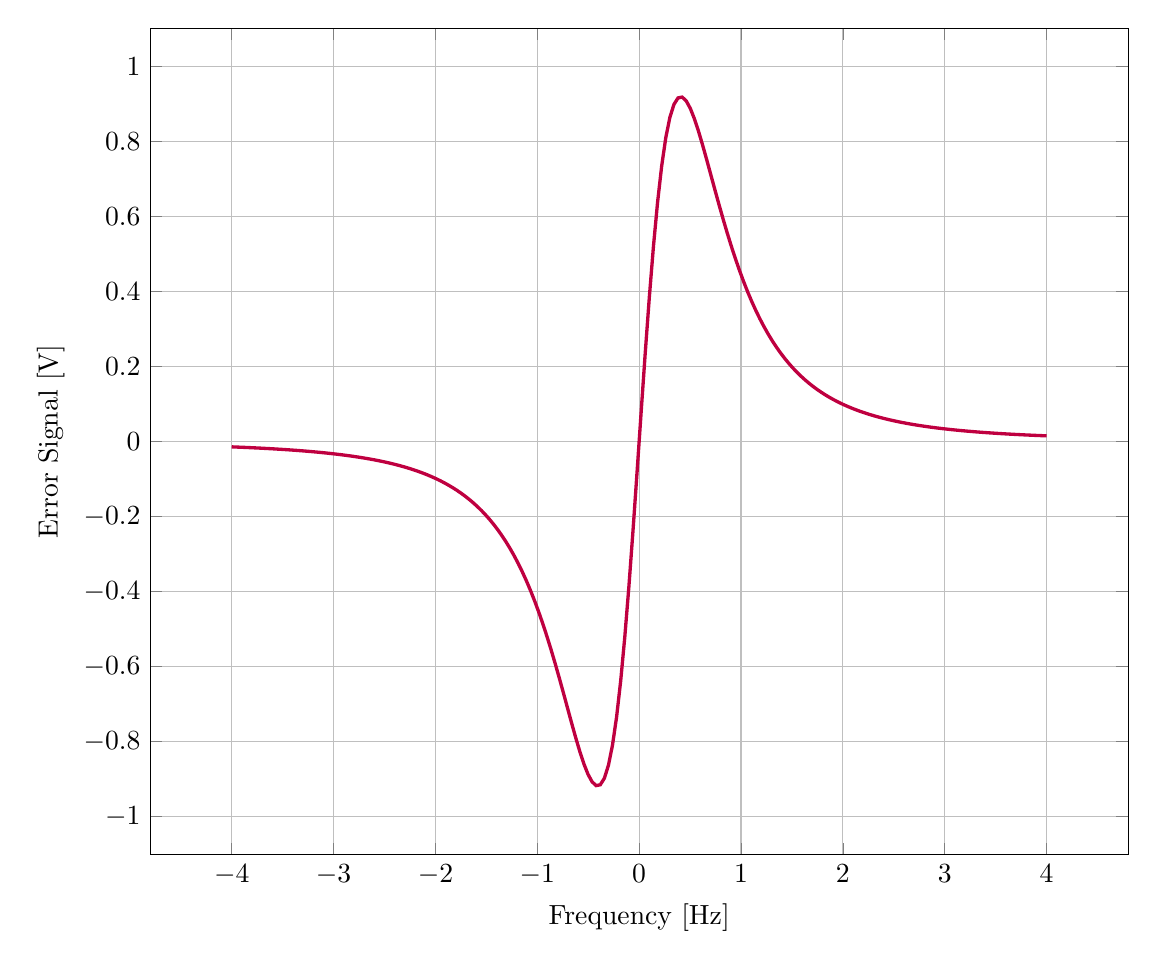
\begin{tikzpicture}
\begin{axis}[
    samples=200,
    grid=both,
    xlabel={Frequency $\left[\mathrm{Hz}\right]$},
    ylabel={Error Signal $\left[\mathrm{V}\right]$}
    ]
%  \addplot[blue,domain=-4:4,very thick] {x*exp(-x*x)};
  \addplot[purple,domain=-4:4,very thick] {x/(x*x+0.5)/(x*x+0.5)};
\end{axis}
\end{tikzpicture}
\caption[PDH Error Signal]{This shows the \ac{pdh} error signal of a simple
  cavity.
  Our lock point must be between the positive and negative cavity poles
  (maximum  and minimum on the y-axis).
  }
\label{fig:pdh}
\end{figure}

\subsubsection{Cavity Assembly}

The reference cavity is a Fabry Perot made from an 8 inch monolithic fused silica
spacer with high reflectivity mirrors glued onto the ends. The reflectivity
of the mirrors yield a finesse of about 7600. Finesse is defined as the ratio
of the \ac{fsr} to the cavity linewidth (\ac{fwhm}). One can arrive the
relationships between FSR, Finesse, mirror reflectivity as follows,
\begin{align}
E_{\mathrm{cavity}} =& E_{\mathrm{incident}} \sqrt{1-r_1^2} \left( 1 + r_1 r_2
    e^{i \omega 2 L /c} + \left(1+r_1 r_2 e^{i \omega 2L/c} \right)^2 + \ldots \right)
    \\
=& E_{\mathrm{incident}} \sqrt{1-r_1^2} \left( \frac{1}{1 - r_1 r_2
    e^{i \omega 2L/c}} \right)
\end{align}
Now, we find the reflected field,
\begin{align}
E_{\mathrm{reflected}} =& E_{\mathrm{incident}} \left( 1-r_1^2 \right)
    \left( \frac{r_2 e^{i \omega 2L/c}}{1 - r_1 r_2 e^{i \omega 2L/c}} \right)
    - r_1 E_{\mathrm{incident}}
\end{align}

\subsubsection{Cavity Suspension}
\begin{figure}[htbp]
	\centering
		\includegraphics[width=15cm]{./figures/refcavsusdesign.pdf}
	\caption[Reference Cavity Suspension Design]{Design of the reference cavity suspension}
	\label{fig:refcav_sus}
\end{figure}


\subsection{Feedback}
The feedback electronics used for the \ac{fss} are from initial LIGO. The board
provides feedback signal for 2 different actuation paths. The low frequency path
is to the laser cavity length which is split again into two different actuation
paths (thermal control and a piezo electric transducer in the laser head). The
other path is to an \ac{eom} to actuate on the phase of the laser beam.

\subsection{Actuation}

There are three actuators. Low frequency actuation is by a thermal controller in
the laser head which actuates on the the cavity length through thermal expansion.
The mid frequency actuation is by \ac{pzt} which applies a force to change the
cavity length. The high frequency actuation is by phase modulation of the light
after it exits the laser head using an \ac{eom}.

%\todopar{Add a description of the Electro-Optic Modulator}

%\subsubsection{Laser Head Thermal}
%
%\subsubsection{Laser Head Piezo-Electric Transducer}
%\todopar{add description of peizo-electric effect}
%\todopar{describe the effects of the piezo in-loop}

\subsubsection{Electro Optic Modulator}

\section{Mode Cleaner}
%\todopar{add description of PMC, reference Willke,98}
The PMC is a ring cavity of three mirrors.
see  \cite{Willke:98}


\subsection{Sensing}

\subsection{Feedback}

\subsection{Actuation}
Actuation on cavity length is done with a piezo-electric transducer on one of
the mirrors. This transducer converts voltage to cavity length.



\Chapter{Linear Trap Experiment}
\label{ch:lintrapex}

\section{Experimental Layout}

\section{High-Q Payload Suspension}

\section{Procedures}

\subsection{Measure the optical losses up to the cavity}

\subsection{Calibration of carrier and subcarrier photodiodes}
We will calibrate the photodiodes while the cavity is not locked, knowing the incident beam power and the round trip losses.

\begin{itemize}
    \item Block carrier light in Mach-Zehnder path.
    \item Turn the reflection monitor beam half-wave plate to minimize subcarrier light on the photodiode.
    \item Block the reflection monitor beam to measure dark voltage at DCPD ($A$).
    \item Unblock the reflection monitor beam and measure voltage at DCPD ($B$).
    \item Unblock the carrier light and measure again ($C$)
    \item Block subcarrier light and measure the carrier power using power meter after last steering mirror on table 1 ($D$).
    \item Using the measured optical loss to the cavity ($L$) compute the mW/mV calibration:
    \begin{itemize}
        \item $\frac{D\cdot L}{C - B}$
    \end{itemize}
\end{itemize}

\section{Mode Matching}
We want to know how much power couples into the cavity from a
perfectly gaussian beam of the wrong size and location. We start with
the equations for the Hermite-Gaussian beam expansion as discussed in
\cite{Siegman86}.

\newcommand{\intinfxy}[1]{\int^{\infty}_{- \infty} \int^{\infty}_{- \infty} #1 \,dx \,dy}
\newcommand{\intinfrt}[1]{\int^{2 \pi}_{0} \int^{\infty}_{0} #1 r \,dr \,d\theta}


\begin{align}
    c_{nm} &= \intinfxy{
    E(x,y,z) u_n^*(x,z)u_m^*(y,z)}
\\  &= \intinfxy{
    E(x,y,z) u_0^*(x,z)u_0^*(y,z)}
\\  &= \intinfxy{
    u_0(x,z-z_0)u_0(y,z-z_0) u_0^*(x,z)u_0^*(y,z)}
\\  &= \intinfxy{ \left( \frac{2}{\pi w^2_0} \right) \left( \frac{q_0}{q(z)} \right)
    \left( \frac{q^*_0}{q^*(z)} \right) \exp \left[-ik \left( x^2 + y^2  \right)
    \left( \frac{1}{2q(z)} + \frac{1}{2q^*(z)} \right) \right]}
\end{align}

Since $q(z) = q_0 + z - z_0$, and $q_0$ is purely imaginary,


\begin{multline}
    c_{00} = \intinfxy{ \left( \frac{2}{\pi w^2_0} \right)
    \left( \frac{-q^2_0}{(q_0+z-z_0)(-q_0+z)} \right) \\
    \exp \left[
    \frac{-ik \left( x^2 + y^2  \right)}{2} \left( \frac{(q_0+z-z_0)-(-q_0+z)}{(q_0+z-z_0)(-q_0+z)} \right)
    \right]}
\end{multline}

A careful analysis of the exponent will reveal that the real part must be greater than $0$.
We can therefore solve the Gaussian integral, setting $s = \frac{-ik \left( x^2 + y^2
\right)}{2} \left( \frac{(q_0+z-z_0)-(-q_0+z)}{(q_0+z-z_0)(-q_0+z)} \right)$

\begin{multline}
    c_{00} = \intinfrt{ \left( \frac{2}{\pi w^2_0} \right)
    \left( \frac{-q^2_0}{(q_0+z-z_0)(-q_0+z)} \right) \\
    \exp \left[
    \frac{-ik \left( r^2  \right)}{2} \left( \frac{(q_0+z-z_0)-(-q_0+z)}{(q_0+z-z_0)(-q_0+z)} \right)
    \right]}
\end{multline}

\begin{align}
    c_{00} &= \intinfrt{ \left( \frac{2}{\pi w^2_0} \right)
    \left( \frac{-q^2_0}{(q_0+z-z_0)(-q_0+z)} \right)
    \exp \left[
    s
    \right]}
\\  &= \int^{\infty}_{0} \left( \frac{4}{w^2_0} \right)
    \left( \frac{-q^2_0}{(q_0+z-z_0)(-q_0+z)} \right)
    \exp \left[
    s
    \right] r \,dr
\\  &= \int^{0}_{-\infty} \left( \frac{4}{w^2_0} \right)
    \left( \frac{-q^2_0}{(q_0+z-z_0)-(-q_0+z)} \right)
    \exp \left[ s
    \right] \frac{1}{-ik} \,ds
\\  &= \left( \frac{4i}{kw^2_0} \right)
    \left( \frac{-q^2_0}{(q_0+z-z_0)-(-q_0+z)} \right)
    \int^0_{-\infty} e^s \,ds
\\  &= \left( \frac{4i}{kw^2_0} \right)
    \left( \frac{-q^2_0}{2q_0-z_0} \right)
\\  &= \left( \frac{4i \lambda}{2 \pi w^2_0} \right)
    \left( \frac{-q^2_0}{2q_0-z_0} \right)
\\  &= \left( \frac{4i \lambda}{2 \pi w^2_0} \right)
    \left( \frac{-q_0 q_b}{2i \pi \omega^2_0 / \lambda - z_0} \right)
\\  &= \left( \frac{4i}{2 \lambda} \right)
    \left( \frac{\pi w_b^2}{2i \pi \omega^2_0 / \lambda - z_0} \right)
\\  &= 
    \frac{w_b^2}{\omega^2_0 + i z_0 \lambda /2 \pi}
\\  &= \frac{(w_b/w_0)^2}{1 + i z_0 /2 z_R}
\end{align}

Power coupling into cavity is then,
\begin{align}
P_{\mathrm{in cavity}} &= P_{\mathrm{incident}} \frac{(w_b/w_0)^4}{1+(z_0/2z_R)^2}
\end{align}



\Chapter{Noise Sources}
\label{ch:noises}
\section{Seismic}

\section{Thermal}

\section{Laser Frequency}

\section{Laser Intensity}

\section{Electronics}

\section{Residual Gas}

\section{Noise Budget}

\begin{figure}[htbp]
	\centering
		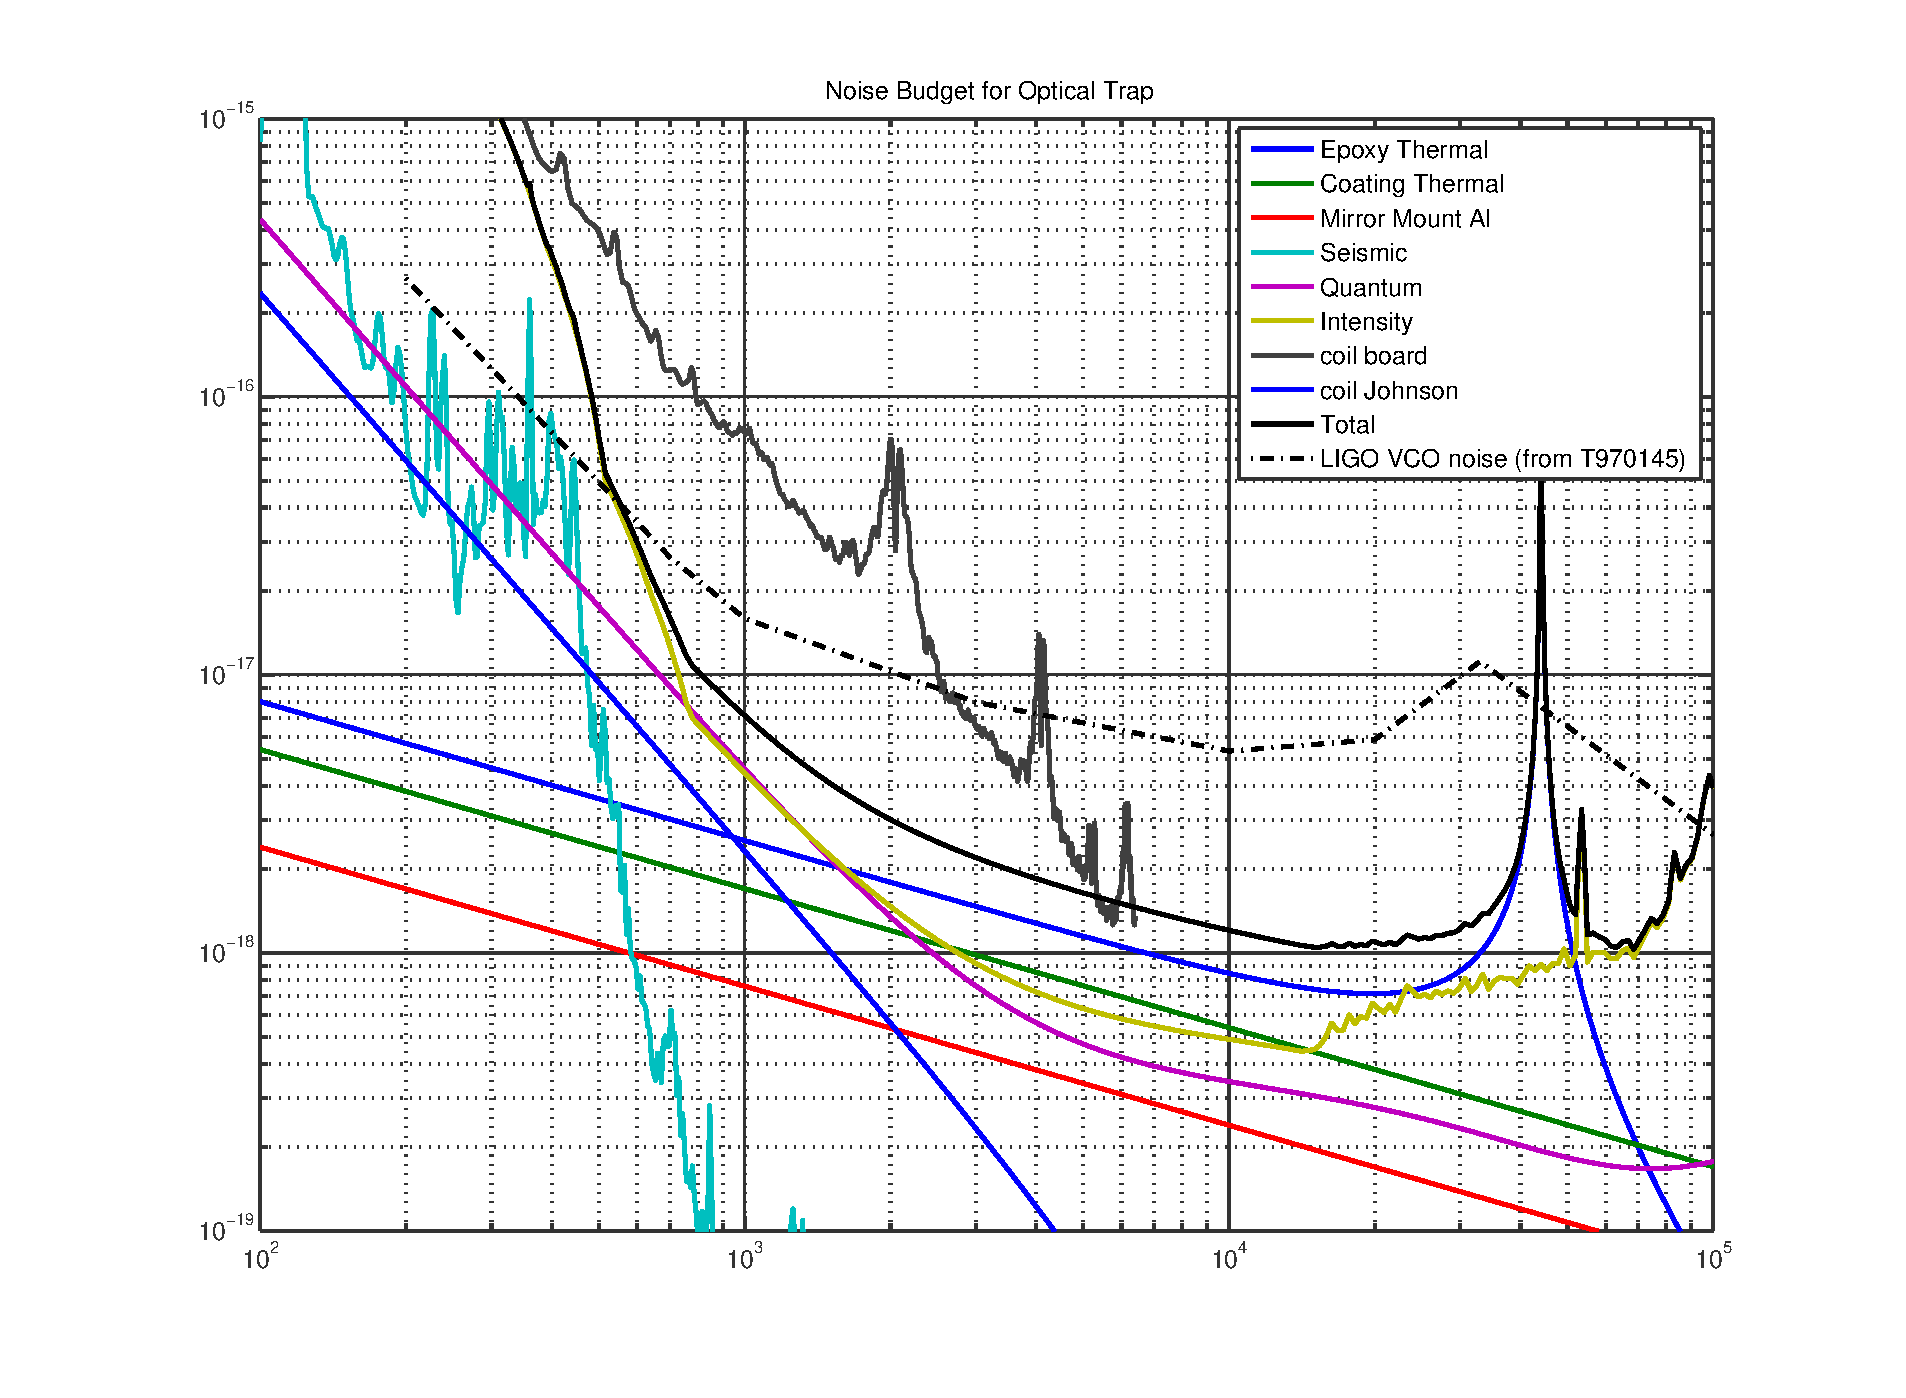
\includegraphics[width=15cm]{./figures/noise_budget.eps}
	\caption[Noise Budget]{Noise budget}
	\label{fig:noise_bud}
\end{figure}

\begin{figure}[htbp]
	\centering
		\includegraphics[width=15cm]{./figures/NoiseBudgetBoard.pdf}
	\caption[Noise Budget Board]{Noise budget with coil driver board noise}
	\label{fig:noise_bud_brd}
\end{figure}

\section{Vacuum Requirements for Optical Trap}

It is desired to have an understanding of limits of vacuum gas constituents for the in-vacuum experiment. From the LIGO DCC we have a few documents that describe the process that went into understanding the problem for 2 4km long Fabry-Perot cavities. I will apply these techniques to a 10-30cm cavity.\\


\subsection{LIGO Vacuum Requirements}

The amplitude spectral density of the optical path length is given by,

\begin{align*}
\Delta L ( f ) = 4 \pi \left( \frac{2 L_0 p}{k T w_0 v_0} \right)^{1/2} a e^{- \pi f w_0 / v_0 }
\end{align*} \\


From *** the value for $4 \pi a \left( \frac{2}{k T w_0 L_0 v_0} \right)^{1/2} $ is $ 4.8 x 10^{-21} \left( \frac{R_x}{R_{H_2}} \right) $. Where $L_0 = 4000 \mathrm{m} $ and $ w_0 = 0.06 \mathrm{m} $. \\

For our purposes (single arm cavity) we will lose a factor of $ \sqrt{2} $. \\

We end up with a formula for amplitude spectral density in a one-arm cavity that is:

\begin{align*}
\Delta L ( f ) = 4 \pi \left( 5.3 \mathrm{x} 10^{-20} \right) \left(  \frac{R_x}{R_{H_2}} \right) \sqrt{\frac{ L_0 p}{ w_0 } } e^{- \pi f w_0 / v_0 }
\end{align*} \\

\subsection{Optical Trap}

Now, we insert parameters for the cavity. For the first look, I use the parameters defined in the project description: 0.3m cavity length, 0.2m radius of curvature for each mirror.
\todo{something},

If we operate at a pressure of 1e-6 Torr, no constituent gas can be greater than this. The following plot is of constituent gases at this pressure.

\begin{figure}[htbp]
	\centering
		\includegraphics[width=15cm]{./figures/trapgasnoise_1.png}
	\caption[Gas Noise Comparison]{Gas Noise for 1e-6 Torr}
	\label{fig:gas_noise1}
\end{figure}

If we have a residual gas analyzer that detects a minimum partial pressure of 5e-11 Torr:

\begin{figure}[htbp]
	\centering
		\includegraphics[width=15cm]{./figures/trapgasnoise_2.png}
	\caption[Gas Noise Comparison]{Gas Noise for 5e-11 Torr}
	\label{fig:gas_noise2}
\end{figure}

\section{Epoxy Thermal Noise}

Brownian thermal noise estimates for epoxy joints are gotten from basic application of the fluctuation-dissipation theorem. The form that we start with is,
\begin{align*}
S_{x^2}(f) = \frac{4 k_B T}{\omega^2} \Re(Z^{-1}), 
\end{align*}
where $Z$ is the impedance, $F / v$. The force equation that we use is of the form,
\begin{align*}
F_{\mathrm{ext}} = m \ddot{x} + k x,
\text{where k is a complex number}, (1 + i \phi)
\end{align*}

\section{Derivation}

\begin{align*}
d_n = d(t-\tau_n)
\end{align*} \\

\begin{align*}
d_n = d \left( t - \frac{(2n -1)}{c} L_0 - d_1 - \sum_{l=2}^{n} 2 d_l \right)
\end{align*} \\



\Chapter{Results}
\label{ch:results}
Linear trap measurements have been taken twice.
The first measurement was with the subcarrier at the same offset frequency from
the carrier for each measurement.
The results generally were in line with the theory, however there were
complications with the layout that we felt should be improved on.

\section{First Experiment}

%\begin{figure}[htbp]
%    \centering
%    \includegraphics[width=20cm]{./figures/april_results_olgfit.eps}
%    \caption[Data Fitting of Open Loop Gain for 1st Results]{This is the open
%        loop gain fit of the last 7 measurements taken during a segment of
%        time in which the cavity was continuously locked.
%        The trap cavity had been locked for a few hours at this point and
%        seemed to have stabilized compared to earlier in the lock segment.
%        These measurements were taken no more than 5 minutes apart from each
%        other so the effects of any drifted were minimized.}
%    \label{fig:olgapril}
%\end{figure}

\begin{figure}[htbp]
  \tikzsetnextfilename{april_olg1}
  \begin{tikzpicture}
  \begin{semilogyaxis}[
    name=plot1,
    height=6cm,
    width=8cm,
    xmin=760,
    xmax=880,
    ylabel={Magnitude},
    grid=major,
  ]
  \addplot[blue] table[x index=0,y index=1] {./matlab_traces/april_olg_38.dat};
  \addplot[blue] table[x index=0,y index=1] {./matlab_traces/april_fit.dat};
  \addplot[red] table[x index=0,y index=1] {./matlab_traces/april_olg_39.dat};
  \addplot[red] table[x index=0,y index=3] {./matlab_traces/april_fit.dat};
  \addplot[green] table[x index=0,y index=1] {./matlab_traces/april_olg_40.dat};
  \addplot[green] table[x index=0,y index=5] {./matlab_traces/april_fit.dat};
  \end{semilogyaxis}

  \begin{semilogyaxis}[
    name=plot2,
    at=(plot1.below south), anchor=above north,
    height=6cm,
    width=8cm,
    xmin=760,
    xmax=880,
    xlabel={Frequency $(H\!z)$},
    ylabel={Magnitude},
    grid=major,
  ]
  \addplot[blue] table[x index=0,y index=1] {./matlab_traces/april_olg_41.dat};
  \addplot[blue] table[x index=0,y index=7] {./matlab_traces/april_fit.dat};
  \addplot[red] table[x index=0,y index=1] {./matlab_traces/april_olg_42.dat};
  \addplot[red] table[x index=0,y index=9] {./matlab_traces/april_fit.dat};
  \addplot[green] table[x index=0,y index=1] {./matlab_traces/april_olg_43.dat};
  \addplot[green] table[x index=0,y index=11] {./matlab_traces/april_fit.dat};
  \addplot[black] table[x index=0,y index=1] {./matlab_traces/april_olg_44.dat};
  \addplot[black] table[x index=0,y index=13] {./matlab_traces/april_fit.dat};
  \end{semilogyaxis}

  \begin{axis}[
    name=plot3,
    at=(plot1.right of east), anchor=left of west,
    height=6cm,
    width=8cm,
    xmin=760,
    xmax=880,
    ylabel={Phase},
    grid=major,
  ]
  \addplot[blue] table[x index=0,y index=2] {./matlab_traces/april_olg_38.dat};
  \addplot[blue] table[x index=0,y index=2] {./matlab_traces/april_fit.dat};
  \addplot[red] table[x index=0,y index=2] {./matlab_traces/april_olg_39.dat};
  \addplot[red] table[x index=0,y index=4] {./matlab_traces/april_fit.dat};
  \addplot[green] table[x index=0,y index=2] {./matlab_traces/april_olg_40.dat};
  \addplot[green] table[x index=0,y index=6] {./matlab_traces/april_fit.dat};
  \end{axis}
  \begin{axis}[
    name=plot4,
    at=(plot2.right of east), anchor=left of west,
    height=6cm,
    width=8cm,
    xmin=760,
    xmax=880,
    xlabel={Frequency $(H\!z)$},
    ylabel={Phase},
    grid=major,
  ]
  \addplot[blue] table[x index=0,y index=2] {./matlab_traces/april_olg_41.dat};
  \addplot[blue] table[x index=0,y index=8] {./matlab_traces/april_fit.dat};
  \addplot[red] table[x index=0,y index=2] {./matlab_traces/april_olg_42.dat};
  \addplot[red] table[x index=0,y index=10] {./matlab_traces/april_fit.dat};
  \addplot[green] table[x index=0,y index=2] {./matlab_traces/april_olg_43.dat};
  \addplot[green] table[x index=0,y index=12] {./matlab_traces/april_fit.dat};
  \addplot[black] table[x index=0,y index=2] {./matlab_traces/april_olg_44.dat};
  \addplot[black] table[x index=0,y index=14] {./matlab_traces/april_fit.dat};
  \end{axis}
  \end{tikzpicture}
    \caption[Data Fitting of Open Loop Gain for 1st Results]{This is the open
        loop gain fit of the last 7 measurements taken during a segment of
        time in which the cavity was continuously locked.
        The trap cavity had been locked for a few hours at this point and
        seemed to have stabilized compared to earlier in the lock segment.
        These measurements were taken no more than 5 minutes apart from each
        other so the effects of any drifted were minimized.}
  \label{fig:aprilolg1}
\end{figure}
\section{Experimental Layout Revision}
From our first layout design there was a rather
large beat signal on the \ac{rfpd} used for generating the \ac{pdh} signal
for our locking feedback servo.
This beat signal is a result of our initial layout involving the combining of
carrier and subcarrier beams before the \ac{fi} which resulted in the two beams
having the same polarization.
This produces a beat signal of the difference in the two frequencies.
The beat signal shows up in our resonant \ac{rfpd} because we use a small
frequency offset.
We feared there could be saturations in the photodiode electronics that would
cause unpredictable electronic offsets in the trap locking feedback servo
resulting in an error on the subcarrier detuning lock point.



\section{Second Experiment}



\Chapter{Conclusions}
\label{ch:conclusions}
%%%%%%%%%%%%%%%%%%%%%%%%%%%%%%%%%%%%%%%%%%%%%%%%%%%%%%%%%%%%%%%%%%%%%%%%%%%%%%%
%%% Describe the wondrous conclusions of the thesis.
%%%%%%%%%%%%%%%%%%%%%%%%%%%%%%%%%%%%%%%%%%%%%%%%%%%%%%%%%%%%%%%%%%%%%%%%%%%%%%%


The first observation runs of Advanced LIGO and Advanced Virgo detectors 
are scheduled for $2015$. By $2018$, these detectors will reach 
their design sensitivity. These second-generation terrestrial detectors
will be able to see up to $10$ times further out in the universe 
than their earlier counterparts. For a compact binary population
uniformly distributed in co-moving volume, this translates to 
a thousandfold increase in the expected detection rate.
% 
Gravitational wave searches make use of theoretical knowledge of
binary dynamics and employ modeled waveforms as filter templates.
With the increase in sensitivity, the resolution of the detectors 
for small errors in modeled waveforms also increases. In this dissertation,
we primarily focus on selecting and developing optimal waveform filters
for Advanced LIGO searches. We also validate gravitational-wave 
search algorithms using accurate numerically simulated signals injected 
into emulated detector noise.

Past binary black hole searches have used post-Newtonian (pN) and 
Effective-One-Body (EOB) waveforms as filters. While the pN waveforms are 
computationally inexpensive, they are restricted to the inspiral
regime of binary coalescence. EOB waveforms include the complete
coalescence process through inspiral, merger and ringdown, and also
the sub-dominant waveform harmonics. However, they are also 
computationally more expensive. For low mass binary black holes 
($m_1,m_2\leq 25M_\odot$),
we explore the region of the parameter space over which pN waveform
templates are sufficiently accurate, in the sense of being able to 
recover more than $97\%$ of the optimal signal-to-noise ratio, 
and where in the parameter space would searches need EOB
waveform templates.
% 
% For binaries with masses $m_1,m_2\leq 25M_\odot$, we compare the 
% inspiral-only post-Newtonian waveforms with the recently proposed
% Effective-One-Body (EOB) model~\cite{BuonannoEOBv2Main}. 
% As this EOB model is calibrated
% against high-accuracy numerical simulations of non-spinning binary 
% black holes, it is demonstrably accurate for {\it comparable}
% mass-ratio binaries. However, it is computationally more expensive
% than the post-Newtonian approximants. 
% We investigate the region of the parameter
% space of non-spinnning binaries where the accuracy of post-Newtonian
% approximants is sufficient and we can win with computational cost, as
% well as the region where EOB waveforms would be required. 
Here we approximate the waveforms with their dominant multipoles. Next,
we study the impact of ignoring sub-dominant waveform multipoles in 
searches. We find that including sub-dominant harmonics could increase
the reach of aLIGO and Virgo for binaries which have their orbital
angular momentum highly inclined to the line of sight connecting them
to the detector.

Numerical Relativity (NR) has seen recent breakthroughs and rapid progress
in simulating the merger of orbiting black holes. These are the most 
accurate solutions to Einstein's field equations available. Still, 
due to their computational cost, numerical relativity simulations 
span only the last stages of the binary inspiral, alongwith the merger
and ringdown. It is possible to join these short but accurate strong-field
simulations with post-Newtonian waveforms that cover the slow-motion
regime, to construct pN-NR {\it hybrids}. We demonstrate that, within 
the limits of current NR technology, it is possible and viable to use 
hybrid waveforms in gravitational wave searches. In addition, we show
that hybrid waveforms can cover the entire region of the binary black
hole parameter space where pN waveforms are insufficient for Advanced 
LIGO searches.


Apart from having applications as search templates, and in enhancing the
accuracy of waveform models, NR simulations
can be used to validate gravitational-wave search algorithms.
We do precisely this within the purview of the NINJA-2 project. 
Several numerical relativity groups contributed
post-Newtonian-hybridized simulations to the project. These were subsequently
injected in emulated advanced detector noise. We demonstrate the ability of
existing search algorithms to successfully {\it detect} these simulations
embedded within realistic noise. This is different from the NINJA-1 project
on a few counts, one of them being the nature of the emulated noise. In the 
NINJA-2 project, initial LIGO data with its non-Gaussian transient noise was
recolored to the expected sensitivity of the Advanced LIGO-Virgo detectors, as
opposed to colored Gaussian noise that was used in NINJA-1. 
Therefore this project provided a more robust test of our search methods, and 
provided a benchmark against which future search developments could be compared.


While the above concerns primarily comparable mass-ratio binaries, we 
also develop a waveform model for intermediate mass-ratio ones with 
$m_1/m_2 \in [10, 100]$. 
Intermediate mass-ratio systems, containing intermediate mass  
and stellar mass black holes will also be relatively more massive than stellar
mass binaries.
This would shift the frequency of the emitted gravitational radiation to 
lower values, and their late-inspiral and merger would occur in the most
sensitive frequency band of the Advanced detectors. This makes the modeling 
of the later portion of their waveforms crucial to their detection. 
%
First-order conservative self-force corrections have been derived for a
test-particle moving in the background of a supermassive Schwarzschild 
black hole. Using the form of these calculations, we formulate a 
prescription to model the early and late inspiral
of such binaries. Then, using the implicit rotation source picture
(due to Baker et al~\cite{Baker:2008}), we develop a model for the plunge and merger,
where the black holes are close and the orbits are no longer quasi-circular.
We then complete the description by stitching the quasi-normal modes emitted
by the black hole formed at merger. 
Therefore, we complete a model that captures the entire coalescence process
for intermediate mass-ratio binaries of non-spinning black holes.

To summarize, for {\it comparable} mass ratio binaries, we show that a combination
of post-Newtonian and post-Newtonian--Numerical-Relativity hybrid waveforms
would be sufficient for gravitational wave searches. This is true for the 
entire stellar-mass non-spinning binary black hole parameter space.
We also successfully validate gravitational wave search algorithms 
that have been used in the most recent LIGO-Virgo searches, using accurate 
numerical simulations injected in emulated detector noise. 
For {\it intermediate} mass ratios, we develop an accurate waveform 
model that captures the binary dynamics from the weak-field slow-motion
regime to the strong-field regime up to the merger of both compact objects. 
Therefore the work presented in this dissertation is an effort towards
arriving at optimal search filters for non-spinning binary black holes 
which are prospective sources detectable by the second-generation terrestrial
gravitational wave detectors; as well as towards validating existing search 
algorithms using an improved testing methodology.














\appendix
\Chapter{Optical Spring Derivation}
\label{ch:otderive}
\section{Optical spring constant derivation}
\label{app:A} 
%\subsection{Optical spring constant}
%\label{sec:Apx1}

In this section we consider the effect of light stored in a detuned Fabry-Perot cavity using a classical approach.
The intra-cavity power generates radiation pressure that exerts on the cavity mirror a force $F_{rad}=-K_{OS}\cdot x$,
where $x$ is the mirror displacement and $K_{OS}$ is the optical spring constant.
Here we show the full derivation of the optical spring constant $K_{OS}$.

We consider a suspended Fabry-Perot cavity of length $L_0$ %shined by a laser light 
with an incident beam of wavelength $\lambda$ and power $P_0$.
First we calculate a general expression of the intra-cavity power and then its  radiation pressure force exerted on the end mirror.\\


\begin{figure}[htbp]
	\centering
		\includegraphics[width=8cm]{./figures/cavity_paper.pdf}
	\caption[Derivation of Optomechanical Cavity Dynamics]{
        A Fabry-Perot cavity of length $L_0$ and coefficients $r_1,t_1$ and $r_2,t_2$ for the input and end mirrors respectively. 
	The input mirror is stationary while the end mirror is affected by harmonic motion. The incoming field $E$ at each round-trip $i$ adds up a phase shift due to the displacement $d_i$}
	\label{fig:cavity_k}
\end{figure}


The field $E=A_0e^{i\omega t}$ enters the cavity through the input mirror of coefficient $t_1=t$ and $r_1$ and the field inside the cavity at the input mirror can be seen as following

\begin{eqnarray}
E_{tot}=E_0+E_1+E_2+E_3+...+En+...
\end{eqnarray}


We consider in our model the following definitions, with $d_n$ being the displacement of the mirror,

\begin{eqnarray}
L_1&=&2(L_0+d_1)\\
L_2&=&2(2L_0+d_1+d_2)\nonumber\\
L_3&=&2(3L_0+d_1+d_2+d_3)\,\, \nonumber\\ %\mbox{with} \,\,d_n=d(t-(2n-1)\tau)\nonumber\\
...\nonumber
\end{eqnarray}
with 
\begin{eqnarray}
\label{eqn:dn1}
d_n &=& d(t-[(2n-1)\tau + \alpha_n ]) \quad \mbox{and}\\
\label{eqn:dn2}
\alpha_n &=& 2\sum\limits_{l=1}^{n-1}\frac{d_l}{c}-\frac{d_n}{c}
\end{eqnarray}

where $\tau=L_0/c$.
With the round trip length $L=2L_0$  we obtain

\begin{eqnarray}
E_{tot}&=&tE(1\!+\!r_1r_2 e^{-ikL_1}\!\!+\!(r_1r_2)^2 e^{-ikL_2}\nonumber\\
&+&(r_1r_2)^3 e^{-ikL_3}  \cdots )\nonumber\\
&=&tE(1\!+\!r_1r_2 e^{-ikL}e^{-2ikd_1}\!\!+\!(r_1r_2)^2 e^{-2ikL}e^{-2ik(d_1\!+\!d_2)}\nonumber\\
&+&(r_1r_2)^3 e^{-3ikL}e^{-2ik(d_1\!+\!d_2\!+\!d_3)}  \cdots )\nonumber
\end{eqnarray}



If we define $X=r_1r_2 e^{-ikL}$ we have 

\begin{eqnarray}
E_{tot}=tE(1+Xe^{-2ikd_1} +X^2e^{-2ik(d_1+d_2)}\nonumber\\
+X^3e^{-2ik(d_1+d_2+d_3)} \cdots )\nonumber
\end{eqnarray}

Since by definition the optical spring $K_{OS}$ is the linear term in the expansion $F=F_0+ K_{OS} d + O(d^2)$, we now expand the exponential in $d_n$. We group  $d_n$ terms:

\begin{eqnarray}
E_{tot}&=&tE(1+X(1-2ikd_1) +X^2(1-2ik(d_1+d_2))\nonumber\\
&+&X^3(1-2ik(d_1+d_2+d_3)) + \cdots )\nonumber \\
\nonumber \\
&=&tE(1+X+X^2+X^3 +\cdots\nonumber\\
&-& 2ikd_1(X+X^2+X^3\cdots)\nonumber\\
&-&2ikd_2(X^2+X^3+X^4\cdots)\nonumber\\  
&-&2ikd_3(X^3+X^4+X^5\cdots)+\cdots) \nonumber \\
\nonumber \\
%&=&tE(\frac{1}{1-X}-2ikd_1\frac{X}{1-X}-2ikd_2\frac{X^2}{1-X}\nonumber \\
%&-&2ikd_3\frac{X^3}{1-X}+\cdots) \nonumber \\
%\nonumber \\
&=&\frac{tE}{1-X}(1-2ikd_1 X-2ikd_2 X^2-2ikd_3 X^3+\cdots) \nonumber
\end{eqnarray}
Since any correction from $\alpha_n$ (equation \ref{eqn:dn2}) is quadratic in $d(t)$, we can again neglect it by definition, and find for the harmonic mirror motion (i.e. in the Fourier domain)
\begin{eqnarray}
d_n&=&x_0e^{i\Omega(t-(2n-1)\tau)}=x_0e^{i\Omega t}e^{-i\Omega(2n-1)\tau}\nonumber\\
&=&x_0e^{i\Omega t} \frac{Y^{2n}}{Y}\frac{Y}{Y}=Y^{2n-2}d_1
\end{eqnarray}

where $Y=e^{-i\Omega\tau}$. Thus we can write


\begin{eqnarray}
E_{tot}&=&\frac{tE}{1-X}(1-2ikd_1 X-2ikd_1 Y^2X^2\nonumber\\
&-&2ikd_1 Y^4 X^3-2ikd_1 Y^6 X^4\cdots)\\
&=&\frac{tE}{1-X}\nonumber\\
&\times &\left[1-2ikd_1 X(1+ Y^2X+ Y^4 X^2+Y^6 X^3\cdots)\right]\nonumber\\
&=&\frac{tE}{1-X}\left [1-\frac{2ikd_1 X}{1-Y^2X}\right ]
\end{eqnarray}

where $d_1$ is a complex number. Since we have to take its real part $Re (d_k)=\frac{d_k+\bar{d}_k}{2}$,
we consider the field inside the cavity with $\bar{d}_k$ conjugate of $d_k$:

\begin{eqnarray}
\frac{tE}{1-X}\left [1-\frac{2ik\bar{d}_1 X}{1-\overline{Y}^2 X}\right ]
\end{eqnarray}

and we obtain as total field $E$

\begin{eqnarray*}
E_{tot}=tE\left [\frac{1}{1-X}- \frac{2ikX}{2(1-X)}   \left ( \frac{d_1}{1-Y^2 X} +\frac{\bar{d}_1}{1-\overline{Y}^2 X}\right )\right]
\end{eqnarray*}

and its complex conjugate 

\begin{eqnarray*}
\overline{E}_{tot}=t\overline{E}\left [\frac{1}{1-\overline{X}}+\frac{2ik\overline{X}}{2(1-\overline{X})}   \left ( \frac{\bar{d}_1}{1-\overline{Y}^2 \overline{X}}+\frac{d_1}{1-Y^2 \overline{X}}\right )\right]
\end{eqnarray*}
 
Using the following expression
 
\begin{eqnarray}
d_1=x_0e^{i\Omega(t-\tau)}=x_0e^{i\Omega t}e^{-i\Omega\tau}=xY  
\end{eqnarray}
 
%Since we are interested only in the linear terms of $d_n$, 
%we neglect $O(d^2)$ terms (\tcb{Stefan could you write a sentence here to say "WHY"?})
we can now obtain the intra-cavity power expression by multiplying $E_{tot}$ by its conjugate
and considering only the linear terms of $x$
%(we neglect $O(d^2)$ terms \tcb{Stefan could you write a sentence here to say "WHY"?})
 
\begin{eqnarray}
P&=&E_{tot}\cdot \overline{E}_{tot}=P_0 t^2[ \frac{1}{(1-X)(1-\overline{X})}\nonumber\\  
&-&\frac{ikX xY}{(1-\overline{X})(1-X)(1-Y^2 X)} -
\frac{ikX \bar{x}\overline{Y}}{(1-\overline{X})(1-X)(1-\overline{Y}^2 X)}\nonumber \\
&+&\frac{ik\overline{X} \bar{x}\overline{Y} } {(1-\overline{X})(1-X)(1-\overline{Y}^2 \overline{X})}+ 
\frac{ik\overline{X} xY}{(1-\overline{X})(1-X)(1-Y^2 \overline{X})}]  \nonumber \\
%\frac{k^2 |X|^2}{4(1-X)(1-\overline{X})} \left( 
%\frac{|x|^2|Y|^2}{(1-Y^2 X)(1-\overline{Y}^2\overline{X})}+
%\frac{|x|^2|Y|^2}{(1-\overline{Y}^2 X)(1-Y^2\overline{X}) }+\nonumber 
%\frac{x^2 Y^2}{(1-Y^2 X)(1-Y^2\overline{X})}+
%\frac{\bar{x}^2 \bar{Y}^2}{(1-\overline{Y}^2 X)(1-\overline{Y}^2\overline{X})}
%\right) ]   
 %\right] 
\end{eqnarray}

where we have also neglected the first constant term. We now group the terms in $x$ and $\bar{x}$:

\newpage
\begin{eqnarray}
%\centering
P&=&-P_0t^2 [ \frac{ikY}{(1-\overline{X})(1-X)} \left( \frac{X}{1-Y^2 X}-\frac{\overline{X}}{1-Y^2\overline{X}} \right) x\nonumber\\
&+&\frac{ik\overline{Y}}{(1-\overline{X})(1-X)} \left( \frac{X}{1-\overline{Y}^2 X}-\frac{\overline{X}}{1-\overline{Y}^2\overline{X}} \right)\bar{x} ]=\nonumber \\
&=&-P_0t^2 [ \frac{ikY}{(1-\overline{X})(1-X)}\nonumber\\ 
&\times &\left( \frac{X}{1-Y^2 X}-\frac{\overline{X}}{1-Y^2\overline{X}} \right) x + cc ]
\end{eqnarray}

Once we have calculated the power we can obtain the radiation pressure force on the end mirror by $F_{rad}=\frac{2 r_2^2}{c}P$. Furthermore
we can also notice the similarity of the expression with the elastic force. Thus we recall that
in frequency domain and complex notation $K$ is defined by $F=-Kx$, the real form is thus

\begin{eqnarray*}
F'=Re[F]=-\frac{1}{2}(Kx+\overline{K}\bar{x})=-\frac{1}{2}(Kx+cc)
\end{eqnarray*}

Taking into account that we are calculating the radiation pressure on the end mirror, we need to consider an extra delay factor $Y$
for the calculation of the power which appears in the expression of $K$. The complex spring is then given by 

\begin{eqnarray*}
%\centering
K=\frac{2 r_2^2}{c} P_0 t^2  \frac{2ikY^2}{(1-\overline{X})(1-X)} \left( \frac{X}{1-Y^2 X}-\frac{\overline{X}}{1-Y^2\overline{X}} \right) 
\end{eqnarray*}
which can be rewritten in the form of equations \ref{KOS_full_2}
and \ref{eqn:K0}.


\subsection*{Detuning}
Given the frequency detuning is $\delta=\omega_0-\omega_{res}$ and $\Omega=\omega-\omega_0$,
where $\omega_0$ is the carrier (sub-carrier) frequency and $\omega_{res}$ is the resonant frequency, we get the following expressions:

\begin{eqnarray}
\mbox{\textit{Resonance}}\nonumber\\ 
\lambda_{res}&=& L/n, \quad k_{res}=\frac{2\pi n}{L}, \nonumber\\ 
\omega_{res} & = & k_{res}\cdot c = \frac{2\pi n}{L} \cdot c\\
\mbox{\textit{Carrier}}\nonumber\\ 
\lambda_0 & = &\lambda,  \quad k_0=\frac{2\pi}{\lambda}=k, \nonumber\\ 
\omega_0 & = & k_0\cdot c=\frac{2\pi c}{\lambda}=w_{res}+\delta\\
\mbox{\textit{Sideband}}\nonumber\\
\omega &=& \Omega+\omega_0=\Omega+\delta+\omega_{res}
\end{eqnarray}

Thus we find
\newpage
\begin{eqnarray}
e^{-ikL}\equiv e^{-ik_0L}=e^{-i\omega_0 \frac{L}{c}}\nonumber\\
=e^{-i(\omega_{res}+\delta)\frac{L}{c}}=e^{-i\omega_{res}\frac{L}{c}}e^{-i\delta\frac{L}{c}}
\end{eqnarray}
Recalling that $\tau=\frac{L_0}{c}=\frac{L}{2c}$ we can write
\begin{eqnarray}
e^{-ikL}=e^{-i\delta 2\tau}%\approx 1-i\delta 2\tau
\end{eqnarray}

%For a negative  detuning
%\begin{eqnarray}
%e^{-ikL} &=& e^{-i(\omega_{res}-\delta)\frac{L}{c}}\nonumber\\
%&=&e^{-i\omega_{res}\frac{L}{c}}e^{i\delta\frac{L}{c}}% \approx 1+i\tau2\delta
%\end{eqnarray}

If we now replace $X$ and $Y$ we obtain the exact expression for $K$:%the most general expression of $K$ that has seen so far 

\begin{eqnarray}
%\centering
K_{OS}=&-P_0 t^2 r_2^2 \frac{4ike^{-2i\Omega\tau}}{c(1-r_1\!r_2e^{i2\delta\tau})(1-r_1\!r_2e^{-i2\delta\tau})}\times\nonumber\\
 & \left( \frac{r_1\!r_2e^{-i\delta \tau}}{1\!-\!r_1\!r_2e^{-2i\Omega\tau} e^{-i2\delta\tau}}
 \!-\!\frac{r_1\!r_2e^{i2\delta\tau}}{1\!-\!r_1\!r_2e^{-2i\Omega\tau}e^{i2\delta\tau}} \right) 
\end{eqnarray}


To compare to existing literature we now expand the exponentials to linear order 
in $\Omega$ and $\delta$, 
$e^{-i\delta 2\tau}\approx 1-i\delta 2\tau$
and $e^{-i2\Omega \tau}\approx 1-i2\Omega \tau$:

\begin{eqnarray}
K =& -P_0 t^2 r_2^2 \times \nonumber\\
& \frac{4ik(1-2i\Omega\tau)r_1r_2}{c(1-r_1r_2+r_1r_2i2\delta\tau)(1-r_1r_2-r_1r_2i2\delta\tau)}\times\\
& \left[\frac{1-i2\delta\tau}{1-r_1r_2(1-2i\Omega\tau-i2\delta\tau)} -\frac{1+i2\delta\tau}{1-r_1r_2(1-2i\Omega\tau+i2\delta\tau)} \right] \nonumber 
\end{eqnarray}

%\begin{eqnarray}
%=-P_0 t^2 r_2^2 \times\nonumber \\
%\frac{4ik(1-2i\Omega\tau)r_1r_2}{c(1+\frac{r_1r_2}{1-r_1r_2}i2\delta\tau)(1-\frac{r_1r_2}{1-r_1r_2}i2\delta\tau)(1-r_1r_2)^3}\nonumber\\
%\left[\frac{1-i\tau2\delta}{1+\frac{r_1r_2}{1-r_1r_2}2i\Omega\tau+\frac{r_1r_2}{1-r_1r_2}i2\delta\tau} -
%\frac{1+i\tau2\delta}{1+\frac{r_1r_2}{1-r_1r_2}2i\Omega\tau-\frac{r_1r_2}{1-r_1r_2}i2\delta\tau}
%\right]\nonumber
%\end{eqnarray}

Considering the $Finesse \approx \pi \frac{r_1r_2}{1-r_1r_2}= \pi FSR/\gamma$, the cavity bandwidth $\gamma$, and the free spectral range $FSR=1/2\tau$, we obtain:

\begin{eqnarray}
K_{OS}\approx-P_0 t^2 r_2^2 \frac{4ik(1-2i\Omega\tau)r_1r_2}{c(1+i\frac{\delta}{\gamma})(1-i\frac{\delta}{\gamma})(1-r_1r_2)^3} \nonumber\\
\times\left[\frac{1-i2\delta}{1+\frac{\Omega}{\gamma}i+\frac{\delta}{\gamma}i} -
\frac{1+i2\delta}{1+\frac{\Omega}{\gamma}i-\frac{\delta}{\gamma}i}
\right]
\end{eqnarray}

Finally, since they correspond to a simple time delay, we neglect the $i\Omega\tau$, $i\delta\tau$ terms in the numerator and obtain
\begin{eqnarray}
K_{OS} & \approx & P_0 t^2 r_2^2 \frac{8k r_1r_2}{c(1-r_1r_2)^3}\frac{ \frac{\delta}{\gamma}}{(1+\frac{\delta^2}{\gamma^2})} 
\left[\frac{1}{1+\frac{\delta^2}{\gamma^2}-\frac{\Omega^2}{\gamma^2}+i2\frac{\Omega}{\gamma} }\right]\nonumber\\
%& = & \frac{K_0}{1+\frac{\delta^2}{\gamma^2}-\frac{\Omega^2}{\gamma^2}+i2\frac{\Omega}{\gamma}}
\end{eqnarray}

\subsubsection{Overcoupled cavity}

In the particular case of perfectly over-coupled cavity ($r_2=1$) $Finesse/\pi=2/T_1$ and $(1-r_1r_2)^2=T_1^2/2$ and the optical spring constant becomes:

\begin{eqnarray}
K_{OS} & \approx & 128 P_0  \frac{\pi}{c\lambda T_1^2}\frac{ \frac{\delta}{\gamma}}{(1+\frac{\delta^2}{\gamma^2})} 
\left[\frac{1}{1+\frac{\delta^2}{\gamma^2}-\frac{\Omega^2}{\gamma^2}+i2\frac{\Omega}{\gamma} }\right]\nonumber\\
\label{eqn:overcoupled}
%& = & \frac{K_0}{1+\frac{\delta^2}{\gamma^2}-\frac{\Omega^2}{\gamma^2}+i2\frac{\Omega}{\gamma}}
\end{eqnarray}

\subsubsection{Matched cavity}

In this case of a matched cavity ($r_1=r_2$) $Finesse/\pi=1/T_1$ and $(1-r_1r_2)^2=T_1^2$ and the optical spring constant remains the same as in Eq.\,\ref{eqn:overcoupled} except for the the factor 128 which has to be replaced with 16.



\section{Torsion pendulum mechanical plant}
\label{app:B} 

Here we transform
the basis of coordinates $\{x_G,\Theta\}$  formed by the position of the center of gravity $x_G$ of the mirror and its rotation angle $\Theta$  with respect to the vertical axis passing from $x_G$ into a basis $\{x_A,x_B\}$ formed by the length of the cavities relative to beam A and beam B respectively. Thus the longitudinal and angular control of the mirror can be treated as the longitudinal control of the two above mentioned cavities. The basis can be expressed as
%
%\begin{eqnarray}
%\label{base}
%x_A = x_G +r_A\Theta \\ \nonumber
%x_B = x_G + r_B\Theta
%\end{eqnarray}

\begin{equation}
\label{eqn:BDEF}
\begin{pmatrix}
x_A \\ x_B
\end{pmatrix}
=
 \begin{pmatrix}
1& r_A\\1& r_B
\end{pmatrix} 
\begin{pmatrix}
x_G\\ \Theta
\end{pmatrix}
=
\mathcal{B}
\begin{pmatrix}
x_G\\ \Theta
\end{pmatrix}
\end{equation}

with $r_A$ and $r_B$ being the lever arms of the two beams with respect to $x_G$.

The equation of motion for the mirror is
\begin{equation}
\label{eqn:motion_matrix}
-\omega^2
\begin{pmatrix}
m &  \\ & I
\end{pmatrix}
 \begin{pmatrix}
x_G\\ \Theta
\end{pmatrix}
= 
\begin{pmatrix}
F_{tot}\\ T_{tot}
\end{pmatrix}
\end{equation}
with $I$ being the moment of inertia of the mirror of mass $m$. We now express the total force and the total torque exerted on the mirror
as function of the individual forces $F_A$ and $F_B$:

\begin{equation}
\label{eqn:FtotTtot}
\begin{pmatrix}
F_{tot} \\ T_{tot}
\end{pmatrix}
=
 \begin{pmatrix}
1& 1\\r_A& r_B
\end{pmatrix} 
\begin{pmatrix}
F_A\\ F_B
\end{pmatrix}
=
\mathcal{B}^{T}
\begin{pmatrix}
F_A\\ F_B
\end{pmatrix}
\end{equation}

Using equations \ref{eqn:FtotTtot} and \ref{eqn:BDEF} in equation \ref{eqn:motion_matrix} we obtain the equation of motion in the ${x_A,x_B}$ basis:
\begin{equation}
-\omega^2
\left[
\mathcal{B}^{T-1}
\begin{pmatrix}
m &  \\ & I
\end{pmatrix}
\mathcal{B}^{-1}
\right ]
 \begin{pmatrix}
x_A\\ x_B
\end{pmatrix} 
=
\begin{pmatrix}
F_{A}\\ F_{B}
\end{pmatrix}
\end{equation}

\section{Stability in two dimensions}
\label{app:C}
The control loop stability in multiple dimensions can be evaluated by considering the one-dimensional open-loop transfer function of every control filter (i.e. optical spring) while all other loops stays closed. Here we calculate these open-loop transfer functions for the two-dimesnional case.

Refering to figure \ref{fig:block_loops}, we inject a signal $F_{xa}=F_{\rm ext}$ into port A. The output at port A is $F_{ya}=F_A$. We close the loop from output B to input B by feeding back the force $F_B$.
%We inject an external signal $n=F_{xa}-F_{ya}$ along the loop A  %as it could be a swept-sine from a network analyser
%to measure the open loop transfer function for cavity A. %while beam B loop remain closed. That can be represented as:
%\begin{equation}
%HM
%\left( \begin{array}{c}
%F_A\\F_B
%\end{array} \right)
%+
%HM
%\left( \begin{array}{c}
%n\\0
%\end{array} \right)
%=
%\left( \begin{array}{c}
%F_{A}\\F_B
%\end{array} \right)
%\end{equation}
%with $n$ being an external signal injected between $F_{xa}$ and $F_{ya}$. %as in practice could
%be a swept-sine injected from a network analyser. 
%Inserting $n=F_{xa}-F_{ya}$ and 
We obtain the following expression:
\begin{equation}
HM
\left( \begin{array}{c}
0\\F_B
\end{array} \right)
+
HM
\left( \begin{array}{c}
F_{xa}\\0
\end{array} \right)
=
\left( \begin{array}{c}
F_{ya}\\F_B
\end{array} \right)
\end{equation}
If we introduce the $2\times2$ matrix $S$: 
\begin{equation}
S_A=
\left( \begin{array}{cc}
0 & 0\\
0 & 1
\end{array} \right)
\end{equation}
we can  write
\begin{equation}
HMS_A
\left( \begin{array}{c}
F_{ya}\\F_B
\end{array} \right)
+
HM
\left( \begin{array}{c}
F_{xa}\\0
\end{array} \right)
=
\left( \begin{array}{c}
F_{ya}\\F_B
\end{array} \right)
\end{equation}
Using the vector $e_A^{T}=(1,0)$ we are able to extract the following open loop
transfer function related to cavity A:
\begin{equation}
OL_{A}=\frac{F_{ya}}{F_{xa}}=e_A^{T}(\mathbb{I}-HMS_A)^{-1}HMe_A
\end{equation}

The same open loop transfer function can be obtained considering an external signal injected into the loop of the beam B while the loop of beam A remains closed.

\begin{equation}
OL_{B}=\frac{F_{yb}}{F_{xb}}=e_B^{T}(\mathbb{I}-HMS_B)^{-1}HMe_B
\end{equation}

with $e_B^{T}=(0,1)$ and % $S_B$:

\begin{equation}
S_B=
\left( \begin{array}{cc}
1 & 0\\
0 & 0
\end{array} \right)
\end{equation}




\Chapter{More Derivations}
\label{ch:moreder}

\section{Mode Matching}
As will be discussed in section
\ref{sec:expimps}, we went through a revision in our overall layout.
This changed the beam size and waist location in reference to the cavity.
We did not want to open the chamber again for alignment and mode matching.
It was useful to know the power coupling into the cavity with the wrong
mode matching to give us an idea of how much transmitted light we should
expect when the cavity is properly aligned since mode matching is a difficult
process of moving the lenses along the beam path and realigning the beam.

We want to know how much power couples into the cavity from a
perfectly gaussian beam of the wrong size and location. We start with
the equations for the Hermite-Gaussian beam decomposition as discussed in
Siegman \cite{Siegman86}. 

\newcommand{\intinfxy}[1]{\int^{\infty}_{- \infty} \int^{\infty}_{- \infty} #1 \,dx \,dy}
\newcommand{\intinfrt}[1]{\int^{2 \pi}_{0} \int^{\infty}_{0} #1 r \,dr \,d\theta}


\begin{align}
    c_{nm} &= \intinfxy{
    E(x,y,z) u_n^*(x,z)u_m^*(y,z)} \nonumber
\\  &= \intinfxy{
    E(x,y,z) u_0^*(x,z)u_0^*(y,z)} \nonumber
\\  &= \intinfxy{
    u_0(x,z-z_0)u_0(y,z-z_0) u_0^*(x,z)u_0^*(y,z)}
\end{align}

We now assign the labels $b$ for the beam and $c$ for the cavity,

\begin{align}
    c_{00} &= \intinfxy{
    u_{b0}(x,z-z_0)u_{b0}(y,z-z_0) u_{c0}^*(x,z)u_{c0}^*(y,z)} \nonumber
\\  &= \intinfxy{ \left( \frac{2}{\pi w^2_0} \right) \left( \frac{q_{b0}}{q_{b}(z)} \right)
    \left( \frac{q^*_{c0}}{q^*_{c}(z)} \right) \exp \left[-ik \left( x^2 + y^2  \right)
    \left( \frac{1}{2q_b(z)} + \frac{1}{2q^*_c(z)} \right) \right]}
\end{align}

Since $q(z) = q_0 + z - z_0$, and $q_0$ is purely imaginary,


\begin{multline}
    c_{00} = \intinfxy{ \left( \frac{2}{\pi w_{b0} w_{c0}} \right)
    \left( \frac{- q_{b0} q_{c0}}{(q_{b0}+z-z_0)(-q_{c0}+z)} \right) \\
    \exp \left[
    \frac{-ik \left( x^2 + y^2  \right)}{2} \left( \frac{(q_{b0}+z-z_0)-(-q_{c0}+z)}{(q_{b0}+z-z_0)(-q_{c0}+z)} \right)
    \right]}
\end{multline}

We start by changing to cylindrical coordinates,

\begin{multline}
    c_{00} = \intinfrt{ \left( \frac{2}{\pi w_{b0} w_{c0}} \right)
    \left( \frac{- q_{b0} q_{c0}}{(q_{b0}+z-z_0)(-q_{c0}+z)} \right) \\
    \exp \left[
    \frac{-ik \left( r^2  \right)}{2} \left( \frac{(q_{b0}+z-z_0)-(-q_{c0}+z)}{(q_{b0}+z-z_0)(-q_{c0}+z)} \right)
    \right]}
\end{multline}

A careful analysis of the exponent will reveal that the real part must be less than $0$.
We can therefore solve the Gaussian integral, setting $s =
\frac{-ik \left( r^2  \right)}{2} \left( \frac{(q_{b0}+z-z_0)-(-q_{c0}+z)}{(q_{b0}+z-z_0)(-q_{c0}+z)} \right)
$,

\begin{align}
    c_{00} &= \intinfrt{ \left( \frac{2}{\pi w_{b0} w_{c0}} \right)
    \left( \frac{- q_{b0} q_{c0}}{(q_{b0}+z-z_0)(-q_{c0}+z)} \right)
    \exp \left[ s
    \right]} \nonumber
\\  &= \int^{\infty}_{0} \left( \frac{4}{w_{b0} w_{c0}} \right)
    \left( \frac{- q_{b0} q_{c0}}{(q_{b0}+z-z_0)(-q_{c0}+z)} \right)
    \exp \left[ s
    \right] r \,dr
\end{align}

Now we transform the differential and the limits of integration, remembering
that the real part of $s$ is less than $0$, $ds =
-ik \left( \frac{(q_{b0}+z-z_0)-(-q_{c0}+z)}{(q_{b0}+z-z_0)(-q_{c0}+z)} \right) r \,dr
$,

\begin{align}
    c_{00} &= \left( \frac{4i}{k w_{b0} w_{c0}} \right)
    \left( \frac{- q_{b0} q_{c0}}{(q_{b0}+z-z_0)-(-q_{c0}+z)} \right)
    \int^{0}_{-\infty} e^s \,ds \nonumber
\\  &= \left( \frac{4i}{k w_{b0} w_{c0}} \right)
    \left( \frac{- q_{b0} q_{c0}}{(q_{b0}+z-z_0)-(-q_{c0}+z)} \right) \nonumber
\\  &= \left( \frac{4i}{k w_{b0} w_{c0}} \right)
    \left( \frac{- q_{b0} q_{c0}}{(q_{b0}+q_{c0}-z_0)} \right)
\end{align}

Now, we rewrite the coefficient in terms of waist sizes and distance between waists, using,
\begin{align*}
    q_0 &= \frac{i \pi w_0^2}{\lambda}
\\  k &= 2 \pi / \lambda
\end{align*}

\begin{align}
    c_{00} &= \frac{2 w_{b0} w_{c0}}{w_{b0}^2 + w_{c0}^2 + i z_0 \lambda / \pi} \nonumber
\\  &= \frac{2 w_{b0} / w_{c0}}{1 + \left( w_{b0} /w_{c0} \right)^2 + i z_0 / z_R}
\end{align}

Power coupling into cavity is then (assuming no loss and $r_1 = r_2$),

%\begin{align}
%    P_{mathrm{trans}} &= P_{mathrm{incident}} \frac{}{}
%\end{align}

\begin{align}
    P_{\mathrm{trans}}  &= P_{\mathrm{incident}} \frac{4 w_{b0}^2 / w_{c0}^2}{1 +
    2 \left( w_{b0} /w_{c0} \right)^2 + \left( w_{b0} /w_{c0} \right)^4 + \left(
    z_0 / z_R \right)^2} \nonumber
\\  P_{\mathrm{trans}}  &= P_{\mathrm{incident}} \frac{4}{ 2 + \left( w_{c0} /
    w_{b0} \right)^2 + \left( w_{b0} /w_{c0} \right)^2 + \left(
    z_0 / z_R \right)^2}
\\  P_{\mathrm{trans}}  &= P_{\mathrm{incident}} \frac{4}{ \left( w_{c0} /
    w_{b0} + w_{b0} / w_{c0} \right)^2 + \left( z_0 / z_R \right)^2}
    \label{eq:symetricmatch}
\end{align}

In equation \ref{eq:symetricmatch} we can see readily the symmetry between
$w_{b0}$ and $w_{c0}$, and the symmetry of $z_0$ about $0$, as expected.


\Chapter{Digital System}
\label{ch:digital}

\section{System Overview}

\begin{figure}[htbp]
	\centering
		\includegraphics[width=15cm]{./figures/FrontEndSystem.pdf}
	\caption{{Front End System Overview}}
	\label{fig:front_end}
\end{figure}


\section{LIGO Real-Time System}

\section{ADC/DAC}

\section{Timing}

The timing signal for the front end system is directly generated by a Stanford Research DS345 function generator. It produces a 65,536 Hz signal that clocks the ADC and DAC cards. Over a long period of time the time stamp in the front end can drift relative to the computers that are synced to network time. Some software, particularly Diagnostic Test Tools and probably others, gets confused when the current time in front end does not match network time. This requires a reboot of the front end system to reacquire the correct time.

We ordered a GPS receiver (Trimble Thunderbolt E) that will prevent these long term drifts. It produces a 1PPS (Pulse Per Second) signal and a 10 MHz signal. The 1PPS connects to the ADC card through the ADC adapter card which is located in the blue expansion chassis. The 10 MHz signal connects to the external timebase input of the DS345. So, the 65,536 clock is now "disciplined" to the GPS time and as such should not drift over long periods of time.

Additionally, the Thunderbolt has an ovenized crystal oscillator that should help with phase noise.

In order to get the GPS antenna signal we needed about 250' of low-loss 1/2" diameter foam core cable (should be easy to spot as it's quite thick). The cable runs out the optics lab, across the hallway overhead and into a cable tray to go down the hallway. The cable runs out of the cable tray by the machine shop, over the hallway, into the machine shop, up to the ceiling, and then along the top of a black drain pipe to the south-east corner of the building. The cable then goes through some grating on the wall and up the shaft to the ground level of the SE corner where the antenna is mounted. (see Fig.\ref{fig:gps_antenna})

\begin{figure}[htbp]
	\centering
		\includegraphics[width=15cm]{./figures/IMG_1308.jpg}
	\caption{{GPS Antenna Location}}
	\label{fig:gps_antenna}
\end{figure}

The 1PPS signal from the Trimble Thunderbolt GPS receiver is a fixed pulse width of 10 micro-seconds. Since the clock is running at 65,536 Hz, the 1PPS is missed by the ADC.

I have fixed this by extending the pulse to about 15 microseconds using a 555 timer chip in monostable mode. The input has to be an inverse pulse so I inverted the pulse in GPS control software. This option is available in the Timing Receiver Configuration window.

See attached NE555P spec sheet (p.9) for the schematic that I used. Only difference is R\_L is between output and ground instead of V\_CC.

I scavenged a 5V power supply from an old 10baseT ethernet hub. I took the ferrites and electrolytic capacitor that were on the supply input in the hub itself and added them to this board for noise suppression.

R\_A is a small potentiometer. If you need to adjust the pulse width, just open the case and turn the pot. Clockwise increases the width.

\begin{figure}[htbp]
	\centering
		\includegraphics[width=15cm]{./figures/timer555.png}
	\caption{{555 Timer Diagram}}
	\label{fig:timer_diag}
\end{figure}


\begin{figure}[htbp]
	\centering
		\includegraphics[width=15cm]{./figures/IMG_1345.jpg}
	\caption{{GPS Pulse Extender}}
	\label{fig:gps_pulse}
\end{figure}

The first thing to check in the GPS software is the status. It should say "over-determined clock". Other key items in the control software to pay attention to are basically the number of green lights (in this case 5) and the holdover time in the upper-right window labeled "Timing Receiver Status and Control". If things are working correctly the number of green satellites will typically be 4-5 with the antenna at it's current location. We should also not see any holdover time. When the receiver is not using any satellites it enters a "holdover" state where the oscillator is no longer disciplining. The GPS keeps track of how long it's been in holdover. Going into holdover could indicate a problem in the connection to the GPS antenna.


\section{Hardware Integration}

\section{Code Installation}

We have acquired a clone of the front end disk used at Livingston. The disk was backed up locally (sugar-dev3:/lab/frontend/sata-disk-backups/mnt2 as of 2013/02/18). The disk was adapted for use at Syracuse. The disk failed on 6 Feb 2013. This page documents the second build of the front end at syracuse...




\section{Using LLO clone disk}



\subsection{LLO tar deploy}

Using the tar file from LLO...

\subsubsection{Local Disk Install}

\subsubsection{Diskless Node Install}

\begin{itemize}
    \item Acquire machine with same architecture as front-end (presumably x86\_64).
    \item Login using gentoo minimal-CD or Live-DVD.
    \item Repartition first disk (/dev/sda) to one partition and create ext3 filesystem.
    \item Make mount point for sda1 and mount.
%
\begin{lstlisting}
mkdir /mnt/fe
mount /dev/sda1 /mnt/fe
\end{lstlisting}
%
    \item Make mount point for /lab and mount directory.

\begin{lstlisting}
mkdir /mnt/lab
mount -t nfs 10.20.1.15:/sugwg/projects/lab /mnt/lab
\end{lstlisting}

    \item copy tar file:

\begin{lstlisting}
rsync -a /mnt/lab/frontend/sata-disk-backups/mnt2/fe.tar.gz /mnt/fe/
\end{lstlisting}

    \item untar file:

\begin{lstlisting}
cd /mnt
tar -xvf fe/fe.tar.gz
\end{lstlisting}

    \item chroot into new filesystem and setup for use on network...
\end{itemize}


\subsection{Minimal tar deploy}

Create a tar file without the portage, front-end target, and cvs/svn directories...

\subsubsection{Creating tar file for Syracuse front-end machine}

This is the procedure used to create an archive of a front-end system modified for use at Syracuse. Here, I am using 10.20.1.44 (s1boot0) as the machine to boot from (the tftp server) and 10.20.1.45 (s1labfe1) is the diskless front-end machine. This can easily be modified for installation directly onto the hard drive.

\begin{enumerate}
    \item Copy the fe tar file to \$\{FE\_LOCATION\} and untar.
\begin{lstlisting}
cd ${FE_LOCATION}
cp /lab/frontend/sata-disk-backups/mnt2/fe.tar.gz .
tar -xvpf fe.tar.gz
\end{lstlisting}
    \item \$\{FE\_LOCATION\}/fe is now the root directory for the front-end system
\begin{lstlisting}
export FE_ROOT=${FE_LOCATION}/fe
\end{lstlisting}
    \item At LLO the controls user has UID:GID = 1001:1001. Change this to 512:512 for Syracuse. (You must execute this as root)
\begin{lstlisting}
find ${FE_LOCATION} -xdev -user 1001 -print0 | xargs -0 chown 512:512
\end{lstlisting}
    \item Change the lines for controls in the files \$\{FE\_ROOT\}/etc/passwd and \$\{FE\_LOCATION\}/fe/etc/group
    \item Edit \$\{FE\_ROOT\}/etc/ntp.conf: Change "server" and "restrict" lines and comment out "broadcast" line
\begin{lstlisting}
server 10.20.1.25
restrict 10.20.1.0 mask 255.255.255.0 nomodify nopeer notrap
\end{lstlisting}
    \item Comment out entries in \$\{FE\_ROOT\}/etc/conf.d/net and add this line:
\begin{lstlisting}
config_eth4=( "10.20.1.45 netmask 255.255.0.0 broadcast 10.20.255.255" )
\end{lstlisting}
    \item Change ip address found in 3 files in \$\{FE\_ROOT\}/etc/xinetd.d/ from 10.144.0.0/24 to 10.20.1.0/24
    \item Comment out 3 lines in \$\{FE\_ROOT\}/etc/resolve.conf
    \item remove \$\{FE\_ROOT\}/opt/rtcds
\begin{lstlisting}
rm -rf ${FE_ROOT}/opt/rtcds
\end{lstlisting}
    \item Comment out all lines in fstab except for "shm" and add lines for root and lab.
\begin{lstlisting}
echo -e "10.20.1.44:/tftpboot/s1labfe1      /               nfs     sync,hard,intr,rw,nolock,rsize=8192,wsize=8192    0 0" >> ${FE_ROOT}/etc/fstab
echo -e "10.20.1.15:/sugwg/projects/lab     /lab            nfs     sync,hard,intr,rw,nolock,rsize=8192,wsize=8192    0 0\n" >> ${FE_ROOT}/etc/fstab
\end{lstlisting}
    \item Change EPICS\_CA\_ADDR\_LIST in \$\{FE\_ROOT\}/opt/cdscfg directory
\begin{lstlisting}
find /ligo/feback/fe/opt/cdscfg/ -type f -print0 | xargs -0 sed --in-place=.old s/10.144.0/10.20.255/g
\end{lstlisting}
    \item Comment out "source /opt/cdscfg/rtsetup.sh" from \$\{FE\_ROOT\}/home/controls/.bashrc and add the following lines in it's place:
\begin{lstlisting}
export IFO=X2
export ifo=x2
export SITE=TST
export site=tst
export RCG_LIB_PATH=/lab/frontend/controls/git/cds_user_apps/cds/b1/models
export RTCDSROOT=/opt/rtcds/${site}/${ifo}
export NDSSERVER=10.20.1.45:8088
export EPICS_CA_ADDR_LIST="10.20.255.255"
export EPICS_CA_AUTO_ADDR_LIST="NO"
export LD_LIBRARY_PATH=${LD_LIBRARY_PATH}:/lib:/usr/lib:/usr/local/lib:/opt/rtapps/fftw-3.2.2/lib
source /opt/rtapps/epics/etc/epics-user-env.sh
source /opt/rtapps/ldas-tools-1.18.2/etc/ldas-tools-user-env.sh
source /opt/rtapps/libframe-8.11/linux-x86_64/etc/libframe-user-env.sh
source /opt/rtapps/libmetaio-8.2/linux-x86_64/etc/libmetaio-user-env.sh
source /opt/rtapps/gds/etc/gds-user-env.sh
export PATH=${PATH}:/opt/rtapps/dv:/opt/rtcds/${site}/${ifo}/scripts
\end{lstlisting}
\end{enumerate}
\subsubsection{Creating a bootable disk for front-end}

This is how to build a disk that can be installed directly into a front-end machine.

*NOTE* The machine that you build this disk from must have the same type of disk controller as the front-end machine you intend to install this in.

\begin{enumerate}
    \item Locate a spare disk and install in a machine connected to the internal network that you have root access to.
    \item Mount /lab on this machine.
    \item Use fdisk or parted to partition the spare disk.
\begin{lstlisting}
Number  Start   End     Size    Type     File system     Flags
 1      512B    32.0MB  32.0MB  primary  ext2
 2      32.5MB  542MB   510MB   primary  linux-swap(v1)
 3      542MB   1000GB  1000GB  primary  ext4
\end{lstlisting}
    \item Mount /dev/sd* (blank spare disk) at /mnt/fe
\end{enumerate}

%\Chapter{Magic Beans}
%\label{ch:usefulformulas}
%In this appendix I present some basic formulas used throughout this thesis.

\section{Optical Cavities}

We can find the beam spot size on a mirror of a two mirror cavity using,
\begin{equation}
w_1^2=\frac{L\lambda}{\pi}\sqrt{\frac{g_2}{g_1\left(1-g_1g_2\right)}}\;,
\end{equation}
where $g$ is a parameter for a mirror with radius of curvature $R$ in a
cavity of length $L$ and is defined by,
\begin{equation}
g=1-\frac{L}{R}\;.
\end{equation}

\begin{equation}
q(z)=z + i\frac{\pi w_0^2}{\lambda}
\end{equation}

\begin{equation}
\frac{1}{q(z)} = \frac{1}{R(z)} -i \frac{\lambda}{\pi w^2(z)}
\end{equation}




%\Chapter{Feedback Control}
%\label{ch:feedback}
%\input(feedback.tex}


\clearpage
\bibliographystyle{unsrt}
\bibliography{OT_paper,references}
\addcontentsline{toc}{chapter}{\numberline {Bibliography}}

\clearpage
\birthplacedate{Blacksburg, Virginia \>\>August 30, 1973}
\collegewherewhen{
\>Virginia Tech \>\>B.S. Physics, 2001}

\newpage
\null%\vskip1in%
\begin{center}
{\Large\bf Vita}
\end{center}

\begin{startvita}
\end{startvita}

\renewenvironment{thebibliography}[1]%
  {\begin{list}{\labelenumi\hss}%
     {\usecounter{enumi}\setlength{\labelwidth}{3em}%
      \setlength{\leftmargin}{5em}}}%
  {\end{list}}
\renewcommand{\bibitem}[1]{\item\label{#1}\relax}%
\renewcommand{\theenumi}{\arabic{enumi}}%
\begin{publications}
\putbib[papers]
\end{publications}


\begin{honorarysocieties}
\end{honorarysocieties}


\end{document}
